\section{Mức độ 7,8 điểm}
\setcounter{ex}{0}
\setcounter{dang}{0}
\Opensolutionfile{ans}[ans/CD1/Muc_7_8]
\begin{dang}{Tìm m để hàm số đơn điệu trên các khoảng xác định của nó}
\end{dang}
\begin{ex}%[2D1K1-1]
	[Đề Tham Khảo Lần 2 2020]%Câu 34
	Có bao nhiêu giá trị nguyên của tham số $ m$ sao cho hàm số $ f(x)=\dfrac{1}{3}{x^3}+m{x^2}+4x+3$ đồng biến trên $\mathbb{R}$.
	\choice
	{\True $ 5$}
	{$ 4$}
	{$ 3$}
	{$ 2$}
	\loigiai{
		Ta có $f'(x)=x^2+2mx+4$.\\
		Hàm số đã cho đồng biến trên $\mathbb{R}$ khi và chỉ khi $f'(x)\ge 0,\forall x\in\mathbb{R}$ (Dấu ``$=$'' xảy ra tại hữu hạn điểm).\\
		Ta có $f'(x)\ge 0,\forall x\in\mathbb{R}\Leftrightarrow\Delta '\le 0$\\
		$\Leftrightarrow\Delta '=m^2-4\le 0$\\
		$\Leftrightarrow-2\le m\le 2$.\\
		Vì $ m\in\mathbb{Z}$ nên $ m\in\left\{-2;-1;0;1;2\right\}$, vậy có $ 5$ giá trị nguyên của $ m$ thỏa mãn.
	}
\end{ex}
\begin{ex}%[2D1K1-1]
	[Mã 123 - 2017]%Câu 35
	Cho hàm số $ y=-x^3-m{x^2}+\left(4m+9\right)x+5$, với $m$ là tham số. Hỏi có bao nhiêu giá trị nguyên của $m$ để hàm số nghịch biến trên khoảng $\left(-\infty ;+\infty\right)$
	\choice
	{$ 5$}
	{$ 4$}
	{$ 6$}
	{\True $ 7$}
	\loigiai{
		Tập xác định $\mathscr{D}=\mathbb{R}$\\
		$ y'=-3x^2-2mx+4m+9$.\\
		Hàm số nghịch biến trên $\left(-\infty ;+\infty\right)$ khi $y'\le 0,\forall x\in\left(-\infty ;+\infty\right)$ $\Leftrightarrow\left\{\begin{aligned}
			& a=-3<0\\ 
			&\Delta '=m^2+3\left(4m+9\right)\le 0\\ 
		\end{aligned}\right.$\\
		$\Leftrightarrow m\in\left[-9;-3\right]$ $\Rightarrow $ có $7$ giá trị nguyên của $m$ thỏa mãn.
	}
\end{ex}
\begin{ex}%[2D1K1-1]%Câu 36
	Cho hàm số $ y=-\dfrac{1}{3}{x^3}+m{x^2}+\left(3m+2\right)x+1$. Tìm tất cả giá trị của $ m$ để hàm số nghịch biến trên $\mathbb{R}$.
	\choice
	{$\left[\begin{aligned}
			& m\ge-1\\ 
			& m\le-2\\ 
		\end{aligned}\right.$}
	{\True $-2\le m\le-1$}
	{$-2<m<-1$}
	{$\left[\begin{aligned}
			& m>-1\\ 
			& m<-2\\ 
		\end{aligned}\right.$}
	\loigiai{
		Tập xác định $\mathscr{D}=\mathbb{R}$, $y'=-x^2+2mx+3m+2$ .\\
		Hàm số nghịch biến trên $\mathbb{R}$ khi và chỉ khi $y'\le 0$, $\forall x\in\mathbb{R}$\\
		$\Leftrightarrow\left\{\begin{aligned}
			& a=-1<0\\ 
			&{\Delta}'=m^2+3m+2\le 0\\ 
		\end{aligned}\right.$ $\Leftrightarrow-2\le m\le-1$.
	}
\end{ex}
\begin{ex}%[2D1K1-1]%Câu 37
	Tìm $ m$ để hàm số $ y=x^3-3m{x^2}+3\left(2m-1\right)+1$ đồng biến trên $\mathbb{R}$.
	\choice
	{Không có giá trị $ m$ thỏa mãn}
	{$ m\ne 1$}
	{\True $ m=1$}
	{Luôn thỏa mãn với mọi $ m$}
	\loigiai{
		$y'=3x^2-6mx+3\left(2m-1\right)$\\
		Ta có $\Delta'=\left(-3m\right)^2-3.3.\left(2m-1\right)$. Để hàm số luôn đồng biến trên $\mathbb{R}$ thì $\Delta'\le 0$\\
		$\Leftrightarrow 9m^2-18m+9<0\Leftrightarrow 9\left(m^2-2m+1\right)\le 0\Leftrightarrow 9\left(m-1\right)^2\le 0$ $\Leftrightarrow m=1$.
	}
\end{ex}
\begin{ex}%[2D1K1-1]%Câu 38
	Tìm điều kiện của tham số thực $ m$ để hàm số $ y=x^3-3x^2+3\left(m+1\right)x+2$ đồng biến trên $\mathbb{R}$.
	\choice
	{$ m\ge 2$}
	{$ m<2$}
	{$ m<0$}
	{\True $ m\ge 0$}
	\loigiai{
		Tập xác định $\mathscr{D}=\mathbb{R}$.\\
		Ta có $y'=3x^2-6x+3\left(m+1\right)$\\
		YCBT $\Leftrightarrow{y}'\ge 0,\forall x\in\mathbb{R}\Leftrightarrow{\Delta}'=-9m\le 0\Leftrightarrow m\ge 0$.
	}
\end{ex}
\begin{ex}%[2D1K1-1]%Câu 39
	Tìm tập hợp tất cả các giá trị của tham số thực $ m$ để hàm số $ y=\dfrac{1}{3}{x^3}+m{x^2}+4x-m$ đồng biến trên khoảng $\left(-\infty ;+\infty\right)$.
	\choice
	{\True $\left[-2;2\right]$}
	{$\left(-\infty ;2\right)$}
	{$\left(-\infty ;-2\right]$}
	{$\left[2;+\infty\right)$}
	\loigiai{
		Ta có $y'=x^2+2mx+4$.\\
		Hàm số đồng biến trên khoảng $\left(-\infty ;+\infty\right)$ khi và chỉ khi $y'\ge 0,\forall x\in\left(-\infty ;+\infty\right)$.\\
		$\Leftrightarrow{\Delta}'=m^2-4\le 0\Leftrightarrow-2\le m\le 2$.
	}
\end{ex}
\begin{ex}%[2D1K1-1]%Câu 40
	Giá trị của $m$ để hàm số $y=\dfrac{1}{3}{x^3}2m{x^2}+\left(m+3\right)x5+m$ đồng biến trên $\mathbb{R}$ là.
	\choice
	{\True $-\dfrac{3}{4}\le m\le 1$}
	{$m\le-\dfrac{3}{4}$}
	{$-\dfrac{3}{4}<m<1$}
	{$m\ge 1$}
	\loigiai{
		Ta có tập xác định $D=\mathbb{R}$.\\
		$y'=x^24mx+\left(m+3\right)$.\\
		$y'=0\Leftrightarrow{x^2}4mx+\left(m+3\right)=0$.\\
		Hàm số đã cho đồng biến trên $\mathbb{R}$ khi và chỉ khi $y'\ge 0,\forall x\in\mathbb{R}$, đẳng thức chỉ xảy ra tại hữu hạn điểm $\Leftrightarrow{\Delta}'\le 0\Leftrightarrow{\left(-2m\right)^2}-1.\left(m+3\right)\le 0\Leftrightarrow 4m^2-m-3\le 0\Leftrightarrow-\dfrac{3}{4}\le m\le 1$.\\
		Vậy $-\dfrac{3}{4}\le m\le 1$.
	}
\end{ex}
\begin{ex}%[2D1K1-1]%Câu 41
	[Chuyên KHTN - Hà Nội - 2020] Tập hợp tất cả các giá trị của tham số $m$ để hàm số $y=x^3+\left(m+1\right){x^2}+3x+2$ đồng biến trên $\mathbb{R}$ là
	\choice
	{\True $\left[-4;2\right]$}
	{$\left(-4;2\right)$}
	{$\left(-\infty ;-4\right]\cup\left[2;+\infty\right)$}
	{$\left(-\infty ;-4\right)\cup\left(2;+\infty\right)$}
	\loigiai{
		Tập xác định: $D=\mathbb{R}$.\\
		Ta có $y'=3x^2+2\left(m+1\right)x+3$.\\
		Hàm số $y=x^3+\left(m+1\right){x^2}+3x+2$ đồng biến trên $\mathbb{R}$ khi và chỉ khi $y'\ge 0,\forall x\in\mathbb{R}$.\\
		$\Leftrightarrow{\Delta}'=\left(m+1\right)^2-9\le 0\Leftrightarrow{m^2}+2m-8\le 0\Leftrightarrow-4\le m\le 2$.\\
		Vậy $ m\in\left[-4;2\right]$.\\
		Nếu hệ số $ a$ chứa tham số thì phải xét trường hợp $ a=0$ và $ a\ne 0$.
	}
\end{ex}
\begin{ex}%[2D1K1-1]
	[Đề Tham Khảo - 2017]%Câu 42
	Hỏi có bao nhiêu số nguyên $ m$ để hàm số $ y=\left(m^2-1\right){x^3}+\left(m-1\right){x^2}-x+4$ nghịch biến trên khoảng $\left(-\infty ;+\infty\right)$.
	\choice
	{$ 0$}
	{$ 3$}
	{\True $ 2$}
	{$ 1$}
	\loigiai{
		Trường hợp 1 $ m=1$. Ta có: $ y=-x+4$ là phương trình của một đường thẳng có hệ số góc âm nên hàm số luôn nghịch biến trên $\mathbb{R}$. Do đó nhận $ m=1$.\\
		Trường hợp 2 $ m=-1$. Ta có: $ y=-2x^2-x+4$ là phương trình của một đường Parabol nên hàm số không thể nghịch biến trên $\mathbb{R}$. Do đó loại $m=-1$.\\
		TH3: $ m\ne\pm 1$. Khi đó hàm số nghịch biến trên khoảng $\left(-\infty ;+\infty\right)$$\Leftrightarrow{y}'\le 0\forall x\in\mathbb{R}$, dấu ``$=$'' chỉ xảy ra ở hữu hạn điểm trên $\mathbb{R}$.\\
		$\Leftrightarrow 3\left(m^2-1\right){x^2}+2\left(m-1\right)x-1\le 0$, $\forall x\in\mathbb{R}$\\
		$\Leftrightarrow\left\{\begin{aligned}
			& a<0\\ 
			&{\Delta}'\le 0\\ 
		\end{aligned}\right.\Leftrightarrow\left\{\begin{aligned}
			&{m^2}-1<0\\ 
			&{\left(m-1\right)^2}+3\left(m^2-1\right)\le 0\\ 
		\end{aligned}\right.\Leftrightarrow\left\{\begin{aligned}
			&{m^2}-1<0\\ 
			&\left(m-1\right)\left(4m+2\right)\le 0\\ 
		\end{aligned}\right.\Leftrightarrow\left\{\begin{aligned}
			&-1<m<1\\ 
			&-\dfrac{1}{2}\le m\le 1\\ 
		\end{aligned}\right.\Leftrightarrow-\dfrac{1}{2}\le m<1$. Vì $m\in\mathbb{Z}$ nên $ m=0$.\\
		Vậy có $2$ giá trị $ m$ nguyên cần tìm là $ m=0$ hoặc $ m=1$.
	}
\end{ex}
\begin{ex}%[2D1K1-1]%Câu 43
	Hỏi có tất cả bao nhiêu giá trị nguyên của tham số $ m$ để hàm số hàm số $ y=\dfrac{1}{3}\left(m^2-m\right){x^3}+2m{x^2}+3x-2$ đồng biến trên khoảng $\left(-\infty ;+\infty\right)$?
	\choice
	{\True $4$}
	{$5$}
	{$3$}
	{$0$}
	\loigiai{
		$y'=\left(m^2-m\right){x^2}+4mx+3$\\
		Hàm số đã cho đồng biến trên khoảng $\left(-\infty ;+\infty\right)$$\Leftrightarrow{y}'\ge 0$ với $\forall x\in\mathbb{R}$.\\
		Với $ m=0$ ta có $y'=3>0$ với $\forall x\in\mathbb{R}$$\Rightarrow $ Hàm số đồng biến trên khoảng $\left(-\infty ;+\infty\right)$.\\
		Với $ m=1$ ta có $y'=4x+3>0\Leftrightarrow x>-\dfrac{3}{4}$ $\Rightarrow $$ m=1$ không thảo mãn.\\
		Với $\left\{\begin{aligned}
			& m\ne 1\\ 
			& m\ne 0\\ 
		\end{aligned}\right.$ ta có $y'\ge 0$ với $\forall x\in\mathbb{R}$$\Leftrightarrow\left\{\begin{aligned}
			&{m^2}-m>0\\ 
			&{\Delta}'=m^2+3m\le 0\\ 
		\end{aligned}\right.$$\Leftrightarrow\left\{\begin{aligned}
			&\left[\begin{aligned}
				& m>1\\ 
				& m<0\\ 
			\end{aligned}\right.\\ 
			&-3\le m\le 0\\ 
		\end{aligned}\right.$$\Leftrightarrow-3\le m<0$.\\
		Tổng hợp các trường hợp ta được $-3\le m\le 0$.\\
		$ m\in\mathbb{Z}\Rightarrow m\in\left\{-3;-2;-1;0\right\}$.\\
		Vậy có $ 4$ giá trị nguyên của $ m$ thỏa mãn bài ra.
	}
\end{ex}
\begin{ex}%[2D1K1-1]%Câu 44
	Tìm tất cả các giá trị của tham số thực $ m$ để hàm số $ y=m{x^3}+m{x^2}+m\left(m-1\right)x+2$ đồng biến trên $\mathbb{R}$.
	\choice
	{$ m\le\dfrac{4}{3}$ và $ m\ne 0$}
	{$ m=0$ hoặc $ m\ge\dfrac{4}{3}$}
	{\True $ m\ge\dfrac{4}{3}$}
	{$ m\le\dfrac{4}{3}$}
	\loigiai{
		Trường hợp 1 $ m=0\Rightarrow y=2$ là hàm hằng nên loại $ m=0$.\\
		Trường hợp 2 $ m\ne 0$. Ta có: $y'=3m{x^2}+2mx+m\left(m-1\right)$.\\
		Hàm số đồng biến trên$\mathbb{R}\Leftrightarrow f'(x)\ge 0\forall x\in\mathbb{R}\Leftrightarrow $\\
		$\left\{\begin{aligned}
			&{\Delta}'=m^2-3m^2\left(m-1\right)\le 0\\
			&3m>0\\
		\end{aligned}\right.\Leftrightarrow\left\{\begin{aligned}
			&{m^2}\left(4-3m\right)\le 0\\ 
			& m>0\\ 
		\end{aligned}\right.\Leftrightarrow\left\{\begin{aligned}
			&m\ge\dfrac{4}{3}\\
			&m>0\\
		\end{aligned}\right.\Leftrightarrow m\ge\dfrac{4}{3}$.
	}
\end{ex}
\begin{ex}%[2D1K1-1]%Câu 45
	Có tất cả bao nhiêu giá trị nguyên của tham số $ m$ để hàm số $ y=\dfrac{m}{3}{x^3}-2m{x^2}+\left(3m+5\right)x$ đồng biến trên $\mathbb{R}$.
	\choice
	{$ 4$}
	{$ 2$}
	{$ 5$}
	{\True $ 6$}
	\loigiai{
		Ta có $y'=m{x^2}-4mx+3m+5$.\\
		Với $a=0\Leftrightarrow m=0$ $\Rightarrow{y}'=5>0$ . Vậy hàm số đồng biến trên $\mathbb{R}$.\\
		Với $a\ne 0\Leftrightarrow m\ne 0$ . Hàm số đã cho đồng biến trên $\mathbb{R}$ khi và chỉ khi\\
		$y'\ge 0,\forall x\in\mathbb{R}\Leftrightarrow\left\{\begin{aligned}
			& a>0\\ 
			&\Delta\le 0\\ 
		\end{aligned}\right.$ $\Leftrightarrow\left\{\begin{aligned}
			& m>0\\ 
			&{\left(2m\right)^2}-m\left(3m+5\right)\le 0\\ 
		\end{aligned}\right.$\\
		$\Leftrightarrow\left\{\begin{aligned}
			& m>0\\ 
			&{m^2}-5m\le 0\\ 
		\end{aligned}\right.\Leftrightarrow\left\{\begin{aligned}
			& m>0\\ 
			& 0\le m\le 5\\ 
		\end{aligned}\right.\Leftrightarrow 0<m\le 5$.\\
		Vì $ m\in\mathbb{Z}\Rightarrow m\in\left\{ 0;1;2;3;4;5\right\}$.
	}
\end{ex}
\begin{ex}%[2D1K1-1]%Câu 46
	Tìm tất cả các giá trị của $ m$ để hàm số $ y=\left(m-1\right){x^3}-3\left(m-1\right){x^2}+3x+2$ đồng biến biến trên $\mathbb{R}$?
	\choice
	{$ 1<m\le 2$}
	{$ 1<m<2$}
	{\True $ 1\le m\le 2$}
	{$ 1\le m<2$}
	\loigiai{
		Ta có $y'=3\left(m-1\right){x^2}-6\left(m-1\right)x+3$.\\
		Hàm số đã cho đồng biến trên $\mathbb{R}$ khi và chỉ khi $y'\ge 0,\forall x\in\mathbb{R}$$\Leftrightarrow\left[\begin{aligned}
			& m-1=0\\ 
			&\left\{\begin{aligned}
				& m-1>0\\ 
				&{\Delta}'\le 0\\ 
			\end{aligned}\right.\\ 
		\end{aligned}\right.$ $\Leftrightarrow\left[\begin{aligned}
			& m=1\\ 
			&\left\{\begin{aligned}
				& m>1\\ 
				& 9\left(m-1\right)^2-9\left(m-1\right)\le 0\\ 
			\end{aligned}\right.\\ 
		\end{aligned}\right.$$\Leftrightarrow\left[\begin{aligned}
			& m=1\\ 
			&\left\{\begin{aligned}
				& m>1\\ 
				& 1\le m\le 2\\ 
			\end{aligned}\right.\\ 
		\end{aligned}\right.$$\Leftrightarrow 1\le m\le 2$.
	}
\end{ex}
\begin{ex}%[2D1K1-1]
	[THPT Hoàng Hoa Thám-Hưng Yên - 2018]%Câu 47
	Số giá trị nguyên của $ m$ để hàm số $y=(4-m^2){x^3}+(m-2){x^2}+x+m-1$ $(1)$đồng biến trên $\mathbb{R}$ bằng.
	\choice
	{$ 5$}
	{$ 3$}
	{$ 2$}
	{\True $ 4$}
	\loigiai{
		Trường hợp 1 $ 4-m^2=0\Leftrightarrow m=\pm 2$.\\
		$ m=2$ $(1)\Leftrightarrow y=x+1$ $\Rightarrow $ hàm số luôn tăng trên $\mathbb{R}$ $\Rightarrow m=2$ (nhận).\\
		$ m=-2$ $(1)\Leftrightarrow y=-4x^2+x-3$ là hàm số bậc hai nên tăng trên khoảng $\left(-\infty ;\dfrac{1}{8}\right)$, giảm trên khoảng $\left(\dfrac{1}{8};+\infty\right)$$\Rightarrow m=-2$ (loại).\\
		Trường hợp 2 $ 4-m^2\ne 0$.\\
		$y'=3\left(4-m^2\right){x^2}+2\left(m-2\right)x+1$. $\Delta'=\left(m-2\right)^2-3\left(4-m^2\right)$$=4m^2-4m-8$.\\
		hàm số đồng biến trên $\mathbb{R}$ $\Leftrightarrow{y}'\ge 0\forall x\in\mathbb{R}$.\\
		$\Leftrightarrow\left\{\begin{aligned}
			& a>0\\ 
			&\Delta\le 0\\ 
		\end{aligned}\right.$$\Leftrightarrow\left\{\begin{aligned}
			& 4-m^2>0\\ 
			& 4m^2-4m-8\le 0\\ 
		\end{aligned}\right.$$\Leftrightarrow\left\{\begin{aligned}
			& m\in\left(-2;2\right)\\ 
			& m\in\left[-1;2\right]\\ 
		\end{aligned}\right.$$\Leftrightarrow m\in\left[-1;2\right)$. $ m\in\mathbb{Z}$$\Rightarrow m=-1$;$ m=0$; $m=1$.\\
		Vậy có $4$ giá trị nguyên của $m$thỏa yêu cầu bài toán.
	}
\end{ex}
\begin{ex}%[2D1K1-1]
	[Chuyên Hoàng Văn Thụ - Hòa Bình - 2018]%Câu 48
	Số các giá trị nguyên của tham số $m$ trong đoạn $\left[-100;100\right]$ để hàm số $y=m{x^3}+m{x^2}+\left(m+1\right)x-3$ nghịch biến trên $\mathbb{R}$ là:
	\choice
	{$200$}
	{\True $99$}
	{$100$}
	{$201$}
	\loigiai{
		Trường hợp 1 $m=0$. Ta có:\\
		$y=x-3$ có $y'=1>0$ với mọi $x\in\mathbb{R}$ nên hàm số luôn đồng biến trên trên $\mathbb{R}$.\\
		Do đó loại $m=0$.\\
		Trường hợp 2 $m\ne 0$. Ta có: $y'=3m{x^2}+2mx+m+1$, $\Delta'=-2m^2-3m=m\left(-2m-3\right)$\\
		Hàm số nghịch biến trên $\mathbb{R}$ khi và chỉ khi $y'\le 0$ với mọi $x\in\mathbb{R}$\\
		$\Leftrightarrow\left\{\begin{aligned}
			& m<0\\ 
			&{\Delta}'\le 0\\ 
		\end{aligned}\right.$ $\Leftrightarrow\left\{\begin{aligned}
			& m<0\\ 
			& m\left(-2m-3\right)\le 0\\ 
		\end{aligned}\right.$ $\Leftrightarrow\left\{\begin{aligned}
			& m<0\\ 
			&-2m-3\ge 0\\ 
		\end{aligned}\right.$ $\Leftrightarrow m\le-\dfrac{3}{2}$.\\
		Vì $m$ là số nguyên thuộc đoạn $\left[-100;100\right]$ nên $m\in\left\{-2;-3;...;-99;-100\right\}$.\\
		Vậy có $99$ giá trị $m$.
	}
\end{ex}
\begin{ex}%[2D1K1-1]
	[Liên trường Nghệ An - 2020]%Câu 49
	Tổng bình phương của tất cả các giá trị nguyên của tham số $ m$ để hàm số $ y=\left(3m^2-12\right){x^3}+3\left(m-2\right){x^2}-x+2$ nghịch biến trên $\mathbb{R}$là?
	\choice
	{$ 9$}
	{$ 6$}
	{\True $ 5$}
	{$ 14$}
	\loigiai{
		Tập xác định $\mathscr{D}=\mathbb{R}$.\\
		Ta có $y'=9\left(m^2-4\right){x^2}+6\left(m-2\right)x-1$.\\
		Hàm số nghịch biến trên $\mathbb{R}\Leftrightarrow y'\le 0\forall x\in\mathbb{R}$(dấu ``$=$'' xãy ra tại hữu hạn $ x\in\mathbb{R}$)\\
		Trường hợp 1 $m^2-4=0\Leftrightarrow m=\pm 2$.\\
		Với $ m=2$ ta có $ y'=-1\le 0$ $\forall x\in\mathbb{R}$ nên $ m=2$ thỏa mãn.\\
		Với $ m=-2$ ta có $ y'=-24x-1\le 0\Leftrightarrow x\ge-\dfrac{1}{24}$(không thỏa với mọi $ x\in\mathbb{R}$) nên loại $ m=-2$.\\
		Trường hợp 2 $m^2-4\ne 0\Leftrightarrow m\ne\pm 2$. Ta có\\
		$ y'\le 0,\forall x\in\mathbb{R}\Leftrightarrow\left\{\begin{aligned}
			& a=9\left(m^2-4\right)<0\\ 
			&{\Delta'}=9\left(m-2\right)^2+9\left(m^2-4\right)\le 0\\ 
		\end{aligned}\right.\Leftrightarrow\left\{\begin{aligned}
			&-2<m<2\\ 
			& 0\le m\le 2\\ 
		\end{aligned}\right.\Leftrightarrow 0\le m<2\xrightarrow{m\in\mathbb{Z}}m\in\left\{ 0;1\right\}$Vậy $ m\in\left\{0;1;2\right\}\Rightarrow{0^2}+1^2+2^2=5$.
	}
\end{ex}
\begin{ex}%[2D1K1-1]
	[Lý Nhân Tông - Bắc Ninh - 2020]%Câu 50
	Hỏi có bao nhiêu số nguyên $ m$ để hàm số $ y=\left(m^2-1\right){x^3}+\left(m-1\right){x^2}-x+4$ nghịch biến trên khoảng$\left(-\infty;+\infty\right)$.
	\choice
	{\True $2$}
	{$1$}
	{$0$}
	{$3$}
	\loigiai{
		Ta có $y'=3\left(m^2-1\right){x^2}+2\left(m-1\right)x-1$\\
		Hàm số đã cho nghịch biến trên khoảng$\left(-\infty;+\infty\right)\Leftrightarrow{y}'\le 0,\forall x\in\mathbb{R}$\\
		$\Leftrightarrow 3\left(m^2-1\right){x^2}+2\left(m-1\right)x-1\le 0,\forall x\in\mathbb{R}$.\\
		Trường hợp 1 $m^2-1=0\Leftrightarrow m=\pm 1$.\\
		Với $ m=1$, ta được $-1\le 0,\forall x\in\mathbb{R}$ (luôn đúng), suy ra $ m=1$ (nhận).\\
		Với $ m=-1$, ta được $-4x-1\le 0\Leftrightarrow x\ge\dfrac{1}{4}$, suy ra $ m=-1$ (loại).\\
		Trường hợp 2 $m^2-1\ne 0\Leftrightarrow m\ne\pm 1$.\\
		Ta có $\Delta'=\left(m-1\right)^2+3\left(m^2-1\right)=m^2-2m+1+3m^2-3=4m^2-2m-2$.\\
		Để $y'\le 0,\forall x\in\mathbb{R}\Leftrightarrow\left\{\begin{aligned}
			&{m^2}-1<0\\ 
			& 4m^2-2m-2\le 0\\ 
		\end{aligned}\right.\Leftrightarrow\left\{\begin{aligned}
			&-1<m<1\\ 
			&-\dfrac{1}{2}\le m\le 1\\ 
		\end{aligned}\right.\Leftrightarrow-\dfrac{1}{2}\le m<1$.\\
		Tổng hợp lại, ta có tất cả giá trị $ m$ cần tìm là $-\dfrac{1}{2}\le m\le 1$.\\
		Vì $ m\in\mathbb{Z}$, suy ra $ m\in\left\{ 0;1\right\}$, nên có $2$ giá trị nguyên của tham số $ m$.
	}      
\end{ex}
\begin{ex}%[2D1K1-1]
	[Mã 105 - 2017]%Câu 51
	Cho hàm số $ y=\dfrac{mx-2m-3}{x-m}$ với $ m$ là tham số. Gọi $S$ là tập hợp tất cả các giá trị nguyên của $ m$ để hàm số đồng biến trên các khoảng xác định. Tìm số phần tử của $S$ .
	\choice
	{Vô số}
	{\True $ 3$}
	{$ 5$}
	{$ 4$}
	\loigiai{
		$ y'=\dfrac{-m^2+2m+3}{\left(x-m\right)^2}$ hàm số đồng biến trên khoảng xác định khi $-1<m<3$ nên có $3$ giá trị của $m$ nguyên.
	}
\end{ex}
\begin{ex}%[2D1K1-1]
	[Mã 104 - 2017]%Câu 52
	Cho hàm số $y=\dfrac{mx+4m}{x+m}$ với $m$ là tham số. Gọi $S$ là tập hợp tất cả các giá trị nguyên của $m$ để hàm số nghịch biến trên các khoảng xác định. Tìm số phần tử của $S$ .
	\choice
	{$4$}
	{Vô số}
	{$3$}      
	{\True $5$}
	\loigiai{
		$\mathscr{D}=\mathbb{R}\setminus\left\{-m\right\}$; $y'=\dfrac{m^2-4m}{\left(x+m\right)^2}$ .\\
		Hàm số nghịch biến trên các khoảng xác định khi $y'<0,\forall x\in D$ $\Leftrightarrow{m^2}-4m<0$ $\Leftrightarrow 0<m<4$.\\
		Mà $m\in\mathbb{Z}$ nên có $3$ giá trị thỏa mãn.
	}
\end{ex}
\begin{ex}%[2D1K1-1]
	[THPT Hoa Lư A - 2018]%Câu 53
	Có tất cả bao nhiêu số nguyên $ m$ để hàm số $ y=\dfrac{\left(m+1\right)x-2}{x-m}$ đồng biến trên từng khoảng xác định của nó?
	\choice
	{$1$}
	{$0$}
	{\True $2$}
	{$3$}
	\loigiai{
		Tập xác định $\mathscr{D}=\mathbb{R}\setminus\left\{ m\right\}$\\
		$y'=\dfrac{-m^2-m+2}{\left(x-m\right)^2}$.\\
		Để hàm số đồng biến trên từng khoảng xác định của ta cần tìm $ m$ để $y'\ge 0$ trên $\left(-\infty ;m\right)$ và $\left(m;+\infty\right)$ và dấu ``$=$'' chỉ xảy ra tại hữu hạn điểm trên các khoảng đó\\
		ĐK $-m^2-m+2>0$ $\Leftrightarrow-2<m<1$. Vì $m\in\mathbb{Z}$ nên $m=-1,$ $0$.
	}
\end{ex}
\begin{ex}%[2D1K1-1]
	[SGD \& ĐT Bắc Giang - 2018]%Câu 54
	Có bao nhiêu giá trị nguyên của tham số $ m$ để hàm số $ y=\dfrac{x+m^2}{x+4}$ đồng biến trên từng khoảng xác định của nó?
	\choice
	{$ 5$}
	{\True $ 3$}
	{$ 1$}
	{$ 2$}
	\loigiai{
		Tập xác định $\mathscr{D}=\mathbb{R}\setminus\left\{-4\right\}$, $y'=\dfrac{4-m^2}{\left(x+4\right)^2}$.\\
		Để hàm số đồng biến trên từng khoảng xác định của nó thì $ 4-m^2>0\Leftrightarrow-2<m<2$.\\
		Do đó có $ 3$ giá trị nguyên của tham số $ m$ thỏa mãn.
	}
\end{ex}
\begin{ex}%[2D1K1-3]
	[THPT Hà Huy Tập - 2018]%Câu 55
	Tìm tất cả giá trị thực của tham số $ m$ để hàm số $ y=\dfrac{x+2-m}{x+1}$ nghịch biến trên các khoảng mà nó xác định?
	\choice
	{$ m\le 1$}
	{$ m\le-3$}
	{$ m<-3$}
	{\True $ m<1$}
	\loigiai{
		Với $ m=1$ thì hàm số là hàm hằng $\left(\forall x\ne-1\right)$ nên không nghịch biến.\\
		Ta có $y'=\dfrac{m-1}{\left(x+1\right)^2},\forall x\ne-1$.\\
		Hàm số nghịch biến trên từng khoảng của tập xác định khi và chỉ khi $y'<0,$$ x\ne-1$$\Leftrightarrow m<1$.
	}
\end{ex}
\begin{ex}%[2D1K1-3]
	[SỞ GD \& ĐT Yên Bái - 2018]%Câu 56
	Tìm tất cả các giá trị thực của tham số $ m$ để hàm số $ y=\dfrac{mx-4}{x-m}$ nghịch biến trên từng khoảng xác định của nó.
	\choice
	{$\left[\begin{aligned}
			m\le-2\\
			m\ge 2\\
		\end{aligned}\right.$}
	{$-2<m<2$}
	{\True $\left[\begin{aligned}
			m<-2\\
			m>2\\
		\end{aligned}\right.$}
	{$-2\le m\le 2$}
	\loigiai{
		Tập xác định $\mathscr{D}=\left(-\infty ;m\right)\cup\left(m;+\infty\right)$.\\
		Ta có $ y=\dfrac{mx-4}{x-m}\Rightarrow y'=\dfrac{-m^2+4}{\left(x-m\right)^2}$. Vì hàm số nghịch biến trên từng khoảng xác định của nó nên $-m^2+4<0\Leftrightarrow\left[\begin{aligned}
			&m<-2\\
			&m>2\\
		\end{aligned}\right.$.
	}
\end{ex}
\begin{ex}%[2D1K1-3]%Câu 57
	[THCS \& THPT Nguyễn Khuyến - Bình Dương-2018] Tìm tất cả các giá trị thực của $ m$ để hàm số $ y=\dfrac{mx-2}{2x-m}$ đồng biến trên mỗi khoảng xác định
	\choice
	{$\left[\begin{aligned}
			& m\le-2\\ 
			& m\ge 2\\ 
		\end{aligned}\right.$}
	{\True $-2<m<2$}
	{$\left[\begin{aligned}
			& m<-2\\ 
			& m>2\\ 
		\end{aligned}\right.$}
	{$-2\le m\le 2$}
	\loigiai{
		Ta có $y'=\dfrac{-m^2+4}{\left(2x-m\right)^2}$,$\forall x\ne\dfrac{m}{2}$\\
		Hàm số đồng biến trên từng khoảng xác định khi $-m^2+4>0\Leftrightarrow-2<m<2$.
	}
\end{ex}
\begin{dang}{Tìm m để hàm số nhất biến đơn điệu trên khoảng cho trước}
\end{dang}
\begin{ex}%[2D1K1-3]
	[Đề Tham Khảo Lần 1 2020]%Câu 58
	Cho hàm số $ f(x)=\dfrac{mx-4}{x-m}$ ($ m$ là tham số thực). Có bao nhiêu giá trị nguyên của $ m$ để hàm số đã cho đồng biến trên khoảng $\left(0;+\infty\right)$?
	\choice
	{$ 5$}
	{$ 4$}
	{$ 3$}
	{\True $ 2$}
	\loigiai{
		Tập xác định $\mathscr{D}=\mathbb{R}\setminus\left\{ m\right\}$.\\
		Đạo hàm $f'(x)=\dfrac{-m^2+4}{\left(x-m\right)^2}$.\\
		Hàm số đồng biến trên $\left(0;+\infty\right)$ khi và chỉ khi\\
		$f'(x)>0\forall x\in\left(0;+\infty\right)\Leftrightarrow\left\{\begin{aligned}
			&-m^2+4>0\\ 
			& m\notin\left(0;+\infty\right)\\ 
		\end{aligned}\right.\Leftrightarrow\left\{\begin{aligned}
			&-2<m<2\\ 
			& m\le 0\\ 
		\end{aligned}\right.\Leftrightarrow-2<m\le 0$.\\
		Do $ m\in\mathbb{Z}\Rightarrow m=\left\{-1;0\right\}$. Vậy có hai giá trị nguyên của $ m$ thỏa mãn đề bài.
	}
\end{ex}
\begin{ex}%[2D1K1-3]
	[Mã 101 – 2020 – Lần 1]%Câu 59
	Tập hợp tất cả các giá trị thực của tham số $ m$ để hàm số $ y=\dfrac{x+4}{x+m}$ đồng biến trên khoảng $\left(-\infty;-7\right)$ là
	\choice
	{$\left[4;7\right)$}
	{\True $\left(4;7\right]$}
	{$\left(4;7\right)$}
	{$\left(4;+\infty\right)$}
	\loigiai{
		Tập xác định $\mathscr{D}=\mathbb{R}\setminus\left\{-m\right\}$.\\
		Ta có $y'=\dfrac{m-4}{\left(x+m\right)^2}$.\\
		Hàm số đã cho đồng biến trên khoảng $\left(-\infty;-7\right)$ $\Leftrightarrow{y}'>0$, $\forall x\in\left(-\infty;-7\right)$ $\Leftrightarrow\left\{\begin{aligned}
			& m-4>0\\ 
			&-m\notin\left(-\infty;-7\right)\\ 
		\end{aligned}\right.$ $\Leftrightarrow\left\{\begin{aligned}
			& m>4\\ 
			&-m\ge-7\\ 
		\end{aligned}\right.\Leftrightarrow\left\{\begin{aligned}
			& m>4\\ 
			& m\le 7\\ 
		\end{aligned}\right.\Leftrightarrow 4<m\le 7$.
	}
\end{ex}
\begin{ex}%[2D1K1-3]
	[Mã 102 - 2020 - Lần 1]%Câu 60
	Tập hợp tất cả các giá trị thực của tham số $m$ để hàm số $y=\dfrac{x+5}{x+m}$ đồng biến trên khoảng $(-\infty ;-8)$ là
	\choice
	{$(5 ;+\infty)$}
	{\True $(5 ; 8]$}
	{$[5 ; 8)$}
	{$(5 ; 8)$}
	\loigiai{
		Điều kiện $x \neq-m$.
		Ta có $y^{\prime}=\dfrac{m-5}{(x+m)^2}$
		Để hàm số $y=\dfrac{x+5}{x+m}$ đồng biến trên khoảng $(-\infty ;-8)$ thì
		$\left\{\begin{aligned}
			&{y'> 0}\\
			&{- m \notin ( - \infty ; - 8 )}\\
		\end{aligned}\Rightarrow \left\{\begin{aligned}
			&m-5>0 \\
			&-m \geq-8\\
		\end{aligned}\Rightarrow 5<m \leq 8 .\right.\right.$.
	}
\end{ex}
\begin{ex}%[2D1K1-3]
	[Mã 103 – 2020 – Lần 1]%Câu 61
	Tập hợp tất cả các giá trị thực của tham số m để hàm số $ y=\dfrac{x+2}{x+m}$ đồng biến trên khoảng $ (-\infty ;-5)$
	\choice
	{\True $(2;5]$}
	{$[2;5)$}
	{$ (2;+\infty)$}
	{$ (2;5)$}
	\loigiai{
		Tập xác định $\mathscr{D}=\mathbb{R}\setminus\left\{-m\right\}.$\\
		Ta có $ y'=\dfrac{m-2}{(x+m)^2}$\\
		Hàm số đồng biến trên khoảng $ (-\infty ;-5)\Leftrightarrow\left\{\begin{aligned}
			&y'>0\forall x\in (-\infty ;-5)\\
			&-m\notin (-\infty ;-5)\\
		\end{aligned}\right.$$\Leftrightarrow\left\{\begin{aligned}
			&m-2>0\\
			&-m\ge-5\\
		\end{aligned}\right.\Leftrightarrow 2<m\le 5$.
	}
\end{ex}
\begin{ex}%[2D1G1-3]
	[Mã 104-2020 – Lần 1]%Câu 62
	Tập hợp tất cả các giá trị thực của tham số $ m$ để hàm số $y=\dfrac{x+3}{x+m}$ đồng biến trên khoảng $\left(-\infty ;-6\right)$ là
	\choice
	{\True $\left(3;6\right]$}
	{$\left(3;6\right)$}
	{$\left(3;+\infty\right)$}
	{$\left[3;6\right)$}
	\loigiai{
		Hàm số xác định khi: $x+m\ne 0\Leftrightarrow x\ne-m$.\\
		$y=\dfrac{x+3}{x+m}\Rightarrow{y}'=\dfrac{m-3}{\left(x+m\right)^2}$\\
		Hàm số đồng biến trên khoảng $\left(-\infty ;-6\right)$ khi và chỉ khi: $\left\{\begin{aligned}
			&{y}'>0,\forall x\in\left(-\infty ;-6\right)\\ 
			&-m\notin\left(-\infty ;-6\right)\\ 
		\end{aligned}\right.$\\
		$\Leftrightarrow\left\{\begin{aligned}
			& m-3>0\\ 
			&-m\in\left[-6;+\infty\right)\\ 
		\end{aligned}\right.\Leftrightarrow\left\{\begin{aligned}
			& m>3\\ 
			&-m\ge-6\\ 
		\end{aligned}\right.\Leftrightarrow\left\{\begin{aligned}
			& m>3\\ 
			& m\le 6\\ 
		\end{aligned}\right.\Leftrightarrow 3<m\le 6$.\\
		Vậy: $m\in\left(3;6\right]$.
	}
\end{ex}
\begin{ex}%[2D1G1-3]
	[Mã 104 - 2018]%Câu 63
	Có bao nhiêu giá trị nguyên của tham số $ m$ để hàm số $ y=\dfrac{x+2}{x+3m}$ đồng biến trên khoảng $\left(-\infty ;-6\right)$.
	\choice
	{\True $ 2$}
	{$ 6$}
	{Vô số}
	{$ 1$}
	\loigiai{
		Tập xác định $\mathscr{D}=\left(-\infty ;-3m\right)\cup\left(-3m;+\infty\right)$.\\
		Ta có $y'=\dfrac{3m-2}{\left(x+3m\right)^2}$\\
		Hàm số đổng biến trên khoảng $\left(-\infty ;-6\right)$$\Leftrightarrow\left\{\begin{aligned}
			& 3m-2>0\\ 
			&-6\le-3m\\ 
		\end{aligned}\right.\Leftrightarrow\left\{\begin{aligned}
			& m>\dfrac{2}{3}\\ 
			& m\le 2\\ 
		\end{aligned}\right.$$\Leftrightarrow\dfrac{2}{3}<m\le 2$.\\
		Mà $ m$ nguyên nên $ m=\left\{ 1;2\right\}$.
	}
\end{ex}
\begin{ex}%[2D1G1-3]
	[Mã 103 - 2018]%Câu 64
	Có bao nhiêu giá trị nguyên của tham số $m$ để hàm số $ y=\dfrac{x+1}{x+3m}$ nghịch biến trên khoảng $\left(6;+\infty\right)$?
	\choice
	{$ 0$}
	{$ 6$}
	{\True $ 3$}
	{Vô số}
	\loigiai{
		Tập xác định $\mathscr{D}=\mathbb{R} \backslash\{-3 m\} ; y'=\dfrac{3 m-1}{(x+3 m)^2}$.\\
		Hàm số $y=\dfrac{x+1}{x+3 m}$ nghịch biến trên khoảng $(6 ;+\infty)$ khi và chỉ khi\\
		$\begin{aligned}
			& \left\{\begin{aligned}
				&{ y'< 0 } \\
				&{ ( 6 ; + \infty ) \subset \mathscr{D}}\\
			\end{aligned} \Leftrightarrow \left\{\begin{aligned}
				&{ 3 m - 1 < 0 } \\
				&{ - 3 m \leq 6 }\\
			\end{aligned} \Leftrightarrow \left\{\begin{aligned}
				&m<\dfrac{1}{3} \\
				&m \geq-2\\
			\end{aligned} \Leftrightarrow-2 \leq m<\dfrac{1}{3} .\right.\right.\right. \\
			&\text{Vì}~m\in \mathbb{Z}\Rightarrow m\in\{-2 ;-1 ; 0\}.
		\end{aligned}$
	}
\end{ex}
\begin{ex}%[2D1G1-3]
	[Mã 101 - 2018]%Câu 65
	Có bao nhiêu giá trị nguyên của tham số $ m$ để hàm số $ y=\dfrac{x+2}{x+5m}$ đồng biến trên khoảng $\left(-\infty ;-10\right)$?
	\choice
	{\True $ 2$}
	{Vô số}
	{$ 1$}
	{$ 3$}
	\loigiai{
		Tập xác định $\mathscr{D}=\mathbb{R}\setminus\left\{-5m\right\}$.\\
		$y'=\dfrac{5m-2}{\left(x+5m\right)^2}$ .\\
		Hàm số đồng biến trên khoảng $\left(-\infty ;-10\right)$ khi và chỉ khi $\left\{\begin{aligned}
			& 5m-2>0\\ 
			&-5m\in\left[-10;+\infty\right)\\ 
		\end{aligned}\right.$\\
		$\Leftrightarrow\left\{\begin{aligned}
			& m>\dfrac{2}{5}\\ 
			&-5m\ge-10\\ 
		\end{aligned}\right.\Leftrightarrow\dfrac{2}{5}<m\le 2$.\\
		Vì $ m$ nguyên nên $ m\in\left\{ 1;2\right\}$.\\ 
		Vậy có $ 2$ giá trị của tham số $ m$.
	}
\end{ex}
\begin{ex}%[2D1G1-3]
	[Mã 102 - 2018]%Câu 66
	Có bao nhiêu giá trị nguyên của tham số $ m$ để hàm số $ y=\dfrac{x+6}{x+5m}$ nghịch biến trên khoảng $\left(10;+\infty\right)$?
	\choice
	{Vô số}
	{\True $ 4$}
	{$ 5$}
	{$ 3$}
	\loigiai{
		Tập xác định $\mathscr{D}=\mathbb{R}\setminus\left\{-5m\right\}$.\\
		$y'=\dfrac{5m-6}{\left(x+5m\right)^2}$\\
		Hàm số nghịch biến trên $\left(10;+\infty\right)$ khi và chỉ khi $\left\{\begin{aligned}
			&{y}'<0,\forall x\in \mathscr{D}\\ 
			&-5m\notin\left(10;+\infty\right)\\ 
		\end{aligned}\right.$$\Leftrightarrow\left\{\begin{aligned}
			& 5m-6<0\\ 
			&-5m\le 10\\ 
		\end{aligned}\right.$$\Leftrightarrow\left\{\begin{aligned}
			& m<\dfrac{6}{5}\\ 
			& m\ge-2\\ 
		\end{aligned}\right.$.\\
		Mà $ m\in\mathbb{Z}$ nên $ m\in\left\{-2;-1;0;1\right\}$.
	}
\end{ex}
\begin{ex}%[2D1G1-3]
	[Chuyên KHTN - 2020]%Câu 67
	Tập hợp tất cả các giá trị của tham số $ m$ để hàm số $ y=\dfrac{mx-4}{x-m}$ đồng biến trên khoảng $\left(-1;+\infty\right)$ là
	\choice
	{$\left(-2;1\right]$}
	{$\left(-2;2\right)$}
	{\True $\left(-2;-1\right]$}
	{$\left(-2;-1\right)$}
	\loigiai{
		Đạo hàm $y'=\dfrac{-m^2+4}{\left(x-m\right)^2}>0,\forall x\ne m$.\\
		Do đó hàm số đồng biến trên $\left(-1;+\infty\right)$ khi $y'>0,\forall x\in\left(-1;+\infty\right)\Leftrightarrow\left\{\begin{aligned}
			&-m^2+4>0\\ 
			& x-m\ne 0,\forall x\in\left(-1;+\infty\right)\\ 
		\end{aligned}\right.\Leftrightarrow\left\{\begin{aligned}
			&-m^2+4>0\\ 
			& x\ne m,\forall x\in\left(-1;+\infty\right)\\ 
		\end{aligned}\right.$ $\Leftrightarrow\left\{\begin{aligned}
			&-2<m<2\\ 
			& m\le-1\\ 
		\end{aligned}\right.\Leftrightarrow-2<m\le-1$.
	}
\end{ex}
\begin{ex}%[2D1G1-3]
	[Chuyên Nguyễn Bỉnh Khiêm - Quảng Nam - 2020]%Câu 68
	Tìm tất cả các giá trị thực của tham số $ m$ để hàm số $ y=\dfrac{mx-1}{m-4x}$ nghịch biến trên khoảng $\left(-\infty ;\dfrac{1}{4}\right)$.
	\choice
	{$ m>2$}
	{\True $ 1\le m<2$}
	{$-2<m<2$}
	{$-2\le m\le 2$}
	\loigiai{
		Tập xác định $\mathscr{D}=\mathbb{R}\setminus\left\{\dfrac{m}{4}\right\}$.\\
		Ta có $y'=\dfrac{m^2-4}{\left(m-4x\right)^2}$.\\
		Hàm số nghịch biến trên khoảng $\left(-\infty ;\dfrac{1}{4}\right)$ khi và chỉ khi $\left\{\begin{aligned}
			&{m^2}-4<0\\ 
			&\dfrac{m}{4}\notin\left(-\infty ;\dfrac{1}{4}\right)\\ 
		\end{aligned}\right.\Leftrightarrow\left\{\begin{aligned}
			&-2<m<2\\ 
			&\dfrac{m}{4}\ge\dfrac{1}{4}\\ 
		\end{aligned}\right.$\\
		$\Leftrightarrow\left\{\begin{aligned}
			&-2<m<2\\ 
			& m\ge 1\\ 
		\end{aligned}\right.\Rightarrow 1\le m<2$.\\
		Vậy $ 1\le m<2$.
	}
\end{ex}
\begin{ex}%[2D1G1-3]%Câu 69
	[Chuyên Thái Nguyên - 2020] Cho hàm số $ y=\dfrac{mx-2m+3}{x+m}$ với $ m$ là tham số. Gọi $ S$ là tập hợp tất cả các giá trị nguyên của $ m$ để hàm số nghịch biến trên khoảng $\left(2;+\infty\right)$. Tìm số phần tử của $ S$.
	\choice
	{$ 5$}
	{\True $ 3$}
	{$ 4$}
	{$ 1$}
	\loigiai{
		Điều kiện xác định $ x\ne-m$.\\
		Ta có $y'=\dfrac{m^2+2m-3}{\left(x+m\right)^2}$.\\
		Để hàm số nghịch biến trên khoảng $\left(2;+\infty\right)$ thì\\
		$\left\{\begin{aligned}
			&{y}'<0;\forall x\in\left(2;+\infty\right)\\ 
			& x\ne-m\\ 
		\end{aligned}\right.$$\Leftrightarrow\left\{\begin{aligned}
			&{m^2}+2m-3<0\\ 
			&-m\le 2\\ 
		\end{aligned}\right.$$\Leftrightarrow\left\{\begin{aligned}
			&-3<m<1\\ 
			& m\ge-2\\ 
		\end{aligned}\right.$$\Leftrightarrow-2\le m<1$.\\
		Vậy giá trị nguyên của $ m$ là $ S=\left\{-2;-1;0\right\}$.
	}
\end{ex}
\begin{ex}%[2D1G1-3]%Câu 70
	[ĐHQG Hà Nội - 2020] Có bao nhiêu giá trị nguyên của tham số $ m$ để hàm số $ y=\dfrac{x+18}{x+4m}$ nghịch biến trên khoảng $\left(2;+\infty\right)$?
	\choice
	{Vô số}
	{$0$}
	{$3$}
	{\True $5$}
	\loigiai{
		Điều kiện $ x\ne-4m$.\\
		Ta có $y=\dfrac{x+18}{x+4m}$$\Rightarrow{y}'=\dfrac{4m-18}{\left(x+4m\right)^2}$.\\
		Hàm số đã cho nghịch biến trên khoảng $\left(2;+\infty\right)$ $\Leftrightarrow\left\{\begin{aligned}
			&{y}'<0\\ 
			&-4m\notin\left(2;+\infty\right)\\ 
		\end{aligned}\right.\Leftrightarrow\left\{\begin{aligned}
			& 4m-18<0\\ 
			&-4m\le 2\\ 
		\end{aligned}\right.\Leftrightarrow\left\{\begin{aligned}
			& m<\dfrac{9}{2}\\ 
			& m\ge-\dfrac{1}{2}\\ 
		\end{aligned}\right.\Leftrightarrow-\dfrac{1}{2}\le m<\dfrac{9}{2}$.\\
		Vì $ m\in\mathbb{Z}$ nên $ m\in\left\{ 0;1;2;3;4\right\}$. Vậy có $5$ giá trị nguyên của tham số $ m$ để hàm số $ y=\dfrac{x+18}{x+4m}$ nghịch biến trên khoảng $\left(2;+\infty\right)$.
	}
\end{ex}
\begin{ex}%[2D1G1-3]
	[Sở Hà Tĩnh - 2020]%Câu 71
	Có bao nhiêu giá trị nguyên của tham số $m$ để hàm số $y=\dfrac{mx+9}{4x+m}$ nghịch biến trên khoảng $\left(0;4\right)$?
	\choice
	{$5$}
	{$11$}
	{\True $6$}
	{$7$}
	\loigiai{
		Điều kiện $x \neq-\dfrac{m}{4}$.\\
		Ta có $y^{\prime}=\dfrac{m^2-36}{(4 x+m)^2}$.\\
		Hàm số đã cho nghịch biến trên khoảng $(0 ; 4) \Leftrightarrow y'<0, \forall x \in(0 ; 4)$.\\
		$\Leftrightarrow\left\{\begin{aligned}
			&{ m ^ { 2 } - 3 6 < 0 } \\
			&{ - \frac { m } { 4 } \notin ( 0 ; 4 ) }
		\end{aligned} \Leftrightarrow \left\{\begin{aligned} 
			&{ - 6 < m < 6 } \\
			&{ [ \begin{aligned} 
					&{ - \dfrac { m } { 4 } \leq 0 } \\
					&{ - \dfrac { m } { 4 } \geq 4 }
			\end{aligned}}
		\end{aligned} \Leftrightarrow \left\{\begin{aligned}
			&-6<m<6 \\
			&{\left[\begin{aligned}
					&m \geq 0 \\
					&m \leq-16
				\end{aligned}\right.}
		\end{aligned} \Leftrightarrow 0 \leq m<6 .\right.\right.\right.$.\\
		Vì $m \in \mathbb{Z}$ nên $m \in\{0,1,2,3,4,5\}$.
		Vậy có $6$ giá trị $m$ thỏa mãn yêu cầu bài toán.
	}
\end{ex}
\begin{ex}%[2D1G1-3]
	[Sở Yên Bái - 2020]%Câu 72
	Tìm tất cả các giá trị thực của tham số $ m$sao cho hàm số $ y=\dfrac{-mx+3m+4}{x-m}$ nghịch biến trên khoảng $\left(1;+\infty\right)$
	\choice
	{$-1<m<4$}
	{\True $-1<m\le 1$}
	{$\left[\begin{aligned}
			& m<-1\\ 
			& m>4\\ 
		\end{aligned}\right.$}
	{$ 1\le m<4$}
	\loigiai{
		$y'=\dfrac{m^2-3m-4}{\left(x-m\right)^2}$\\
		Để hàm số nghịch biến trên khoảng $\left(1;+\infty\right)$ thì $y'<0,\forall x\in\left(1;+\infty\right)$.\\
		$\Leftrightarrow\left\{\begin{aligned}
			&{m^2}-3m-4<0\\ 
			& m\notin\left(1;+\infty\right)\\ 
		\end{aligned}\right.\Leftrightarrow\left\{\begin{aligned}
			& m\in\left(-1;4\right)\\ 
			& m\le 1\\ 
		\end{aligned}\right.\Leftrightarrow-1<m\le 1$.
	}
\end{ex}
\begin{ex}%[2D1G1-3]
	[Đặng Thúc Hứa - Nghệ An - 2020]%Câu 73
	Có bao nhiêu giá trị nguyên của tham số $m\in\left(-2020;2020\right)$ sao cho hàm số $y=\dfrac{3x+18}{x-m}$ nghịch biến trên khoảng $\left(-\infty ;-3\right)$?
	\choice
	{$2020$}
	{$2026$}
	{$2018$}
	{\True $2023$}
	\loigiai{
		Điều kiện $x\ne m$ nên $m\notin\left(-\infty ;-3\right)$\\
		$y=\dfrac{3x+18}{x-m}\Rightarrow y'=\dfrac{-3m-18}{\left(x-m\right)^2}$\\
		Để hàm số $y=\dfrac{3x+18}{x-m}$ nghịch biến trên khoảng $\left(-\infty ;-3\right)$ thì $-3m-18<0\Leftrightarrow m>-6$\\
		Vì $m\in\left(-2020;2020\right)$ và $m\notin\left(-\infty ;-3\right)$ nên $m\in\left[-3;2020\right)$\\
		Vậy có $2023$ giá trị $m$ nguyên thoả mãn.
	}
\end{ex}
\begin{ex}%[2D1G1-3]
	[Lương Thế Vinh - Hà Nội - 2020]%Câu 74
	Có bao nhiêu giá trị nguyên âm của tham số $ m$ để hàm số $ y=\dfrac{x+4}{2x-m}$ nghịch biến trên khoảng $\left(-3;4\right)$.
	\choice
	{Vô số}
	{$ 1$}
	{$ 3$}
	{\True $ 2$}
	\loigiai{
		Tập xác định $\mathscr{D}=\mathbb{R}\setminus\left\{\dfrac{m}{2}\right\}$.\\
		Có $y'=-\dfrac{m+8}{\left(2x-m\right)^2}$\\
		Hàm số nghịch biến trên $\left(-3;4\right)$$\Leftrightarrow{y}'<0\forall x\in\left(-3;4\right)\Leftrightarrow-\dfrac{m+8}{\left(2x-m\right)^2}<0\forall x\in\left(-3;4\right)$\\
		$\Leftrightarrow\left\{\begin{aligned}
			&-\left(m+8\right)<0\\ 
			&\dfrac{m}{2}\notin\left(-3;4\right)\\ 
		\end{aligned}\right.\Leftrightarrow\left\{\begin{aligned}
			& m>-8\\ 
			&\left[\begin{aligned}
				&\dfrac{m}{2}\le-3\\ 
				&\dfrac{m}{2}\ge 4\\ 
			\end{aligned}\right.\\ 
		\end{aligned}\right.\Leftrightarrow\left[\begin{aligned}
			&-8<m\le-6\\ 
			& m\ge 8\\ 
		\end{aligned}\right.$.\\
		Do $ m$ nguyên âm nên $ m\in\left\{-7;-6\right\}$, gồm $ 2$ giá trị thỏa mãn.
	}
\end{ex}
\begin{ex}%[2D1G1-3]%Câu 75
	[Chuyên KHTN - Hà Nội - Lần 3] Có bao nhiêu giá trị nguyên của tham số $ m$ để hàm số $ y=\dfrac{mx+4}{x+m}$ nghịch biến trên khoảng $\left(0;+\infty\right)$?
	\choice
	{$1$}
	{\True $2$}
	{$3$}
	{$5$}
	\loigiai{
		Tập xác định $\mathscr{D}=\mathbb{R}\backslash\left\{-m\right\}$\\
		Ta có $y'=\dfrac{m^2-4}{\left(x+m\right)^2}$.\\
		Hàm số nghịch biến trên khoảng $\left(0;+\infty\right)$ khi và chỉ khi\\
		$\left\{\begin{aligned}
			&{y}'<0,\forall x>0\\ 
			&-m\notin\left(0;+\infty\right)\\ 
		\end{aligned}\right.$ $\Leftrightarrow\left\{\begin{aligned}
			&{m^2}-4<0\\ 
			&-m\le 0\\ 
		\end{aligned}\right.\Leftrightarrow\left\{\begin{aligned}
			&-2<m<2\\ 
			& m\ge 0\\ 
		\end{aligned}\right.\Leftrightarrow 0\le m<2$.\\
		Vậy số giá trị nguyên của tham số $ m$ là $ 2$.
	}
\end{ex}
\begin{dang}{Tìm m để hàm số bậc 3 đơn điệu trên khoảng cho trước}
\end{dang}

\begin{ex}%[Hoàng Thanh Phương, 32CD]%[2D1K1-3]%Câu 6
	Cho hàm số $ y=x^3+3x^2-mx-4$. Tập hợp tất cả các giá trị của tham số $ m$ để hàm số đồng biến trên khoảng $\left(-\infty ;\,0\right)$ là
	\choice
	{$\left(-1;5\right)$}
	{\True $\left(-\infty ;\,-3\right]$}
	{$\left(-\infty ;\,-4\right]$}
	{$\left(-1;\,+\infty\right)$}
	\loigiai{
		Ta có $ y'=3x^2+6x-m$.\\
		Để hàm số đồng biến trên khoảng $\left(-\infty;0\right)$ thì $ y'\ge 0,\, \forall x\in\left(-\infty;0\right)$\\
		$\Leftrightarrow 3x^2+6x-m\ge 0,\,\forall x\in\left(-\infty ;0\right)$\\
		$\Leftrightarrow m\le 3x^2+6x,\,\forall x\in\left(-\infty ;0\right)$.\\
		Đặt $ g(x)=3x^2+6x$, hàm số $ g(x)$ có bảng biến thiên
		\begin{center}
			\begin{tikzpicture}
				\tkzTabInit[nocadre,lgt=1.2,espcl=2.5,deltacl=0.6]
				{$x$/0.6,$y'$/0.6,$y$/2}
				{$-\infty$,$-1$,$0$}
				\tkzTabLine{,-,$0$,+,}
				\tkzTabVar{+/$+\infty$,-/$-3$,+/$0$}
			\end{tikzpicture}
		\end{center}
		Dựa vào bảng biến thiên ta có $\Leftrightarrow m\le 3x^2+6x,\,\forall x\in\left(-\infty ;\,0\right)\Leftrightarrow m\le-3$.
	}
\end{ex}
\begin{ex}%[2D1G1-3]
	[Mã 101 – 2020 - Lần 2]%Câu 76
	Tập hợp tất cả các giá trị thực của tham số $ m$ để hàm số $ y=x^3-3x^2+\left(4-m\right)x$ đồng biến trên khoảng $\left(2;+\infty\right)$ là
	\choice
	{$\left(-\infty ;1\right]$}
	{\True $\left(-\infty ;4\right]$}
	{$\left(-\infty ;1\right)$}
	{$\left(-\infty ;4\right)$}
	\loigiai{
		Ta có\\
		$y'=3x^2-6x+4-m$.$ ycbt\Leftrightarrow{y'}\ge 0,\forall x\in\left(2;+\infty\right)$\\
		$\Leftrightarrow 3x^2-6x+4-m\ge 0,\forall x\in\left(2;+\infty\right)\Leftrightarrow m\le 3x^2-6x+4,\forall x\in\left(2;+\infty\right)$\\
		$\Leftrightarrow m\le\underset{\left(2;+\infty\right)}{\min}g(x)$ với $ g(x)=3x^2-6x+4$\\
		Ta có.\\
		$g(x)=6x-6$\\
		$g(x)=0\Leftrightarrow 6x-6=0\Leftrightarrow x=1$\\
		{\color{red}HÌNH Ở ĐÂY}\\
		Dựa vào bảng biến thiên, suy ra: $ m\le 4$ thỏa yêu cầu bài toán.\\
		Vậy: $ m\in\left(-\infty ;4\right]$ thì hàm số đồng biến trên khoảng $\left(2;+\infty\right)$.
	}
\end{ex}
\begin{ex}%[2D1G1-3]
	[Mã 102 – 2020 – Lần 2]%Câu 77
	Tập hợp tất cả các giá trị của tham số $ m$ để hàm số $ y=x^3-3x^2+\left(5-m\right)x$ đồng biến trên khoảng $\left(2;+\infty\right)$ là
	\choice
	{$\left(-\infty ;2\right)$}
	{$\left(-\infty ;5\right)$}
	{\True $\left(-\infty ;5\right]$}
	{$\left(-\infty ;2\right]$}
	\loigiai{
		Ta có $y'=3x^2-6x+5-m$.\\
		Hàm số đã cho đồng biến trên $\left(2;+\infty\right)$ khi và chỉ khi $y'\ge 0,\forall x\in\left(2;+\infty\right)$\\
		$\Leftrightarrow 3x^2-6x+5-m\ge 0,\forall x>2\Leftrightarrow m\le 3x^2-6x+5,\forall x>2$.\\
		Xét hàm số $ f(x)=3x^2-6x+5$ trên khoảng $\left(2;+\infty\right)$.\\
		Có $f'(x)=6x-6$, $f'(x)=0\Leftrightarrow 6x-6=0\Leftrightarrow x=1$ (loại).\\
		Bảng biến thiên\\
		{\color{red}HÌNH Ở ĐÂY}\\
		Từ bàng biến thiên ta có $ m\le 3x^2-6x+5,\forall x>2$$\Leftrightarrow m\le 5$.\\
		Vậy $ m\in\left(-\infty ;5\right]$.}
\end{ex}
\begin{ex}%[2D1G1-3]
	[Mã 103 – 2020 – Lần 2]%Câu 78
	Tập hợp tất cả các giá trị thực của tham số $ m$để hàm số $ y=x^3-3x^2+\left(2-m\right)x$đồng biến trên khoảng $\left(2;+\infty\right)$là
	\choice
	{$\left(-\infty ;-1\right]$}
	{$\left(-\infty ;2\right)$}
	{$\left(-\infty ;-1\right)$}
	{\True $\left(-\infty ;2\right]$}
	\loigiai{
		Ta có $ y'=3x^2-6x+2-m$.\\
		Để hàm số đồng biến trên khoảng $\left(2;+\infty\right)$ khi và chỉ khi $ y'\ge 0,\forall x\in\left(2;+\infty\right)$\\
		$\Leftrightarrow 3x^2-6x+2-m\ge 0,\forall x\in\left(2;+\infty\right)$$ m\le 3x^2-6x+2,\forall x\in\left(2;+\infty\right)$.\\
		Xét hàm số $ f(x)=3x^2-6x+2,\forall x\in\left(2;+\infty\right)$.\\
		$ f'(x)=6x-6$; $ f'(x)=0\Rightarrow 6x-6=0\Leftrightarrow x=1$.\\
		Bảng biến thiên\\
		{\color{red}HÌNH Ở ĐÂY}\\
		Từ bảng biến thiên ta thấy $ m\le 2$. Vậy $ m\in\left(-\infty ;2\right]$.
	}
\end{ex}
\begin{ex}%[2D1G1-3]
	[Mã 104 – 2020 – Lần 2]%Câu 79
	Tập hợp tất cả các giá trị thực của tham số $ m$ để hàm số $ y=x^3-3x^2+\left(1-m\right)x$ đồng biến trên khoảng $\left(2;+\infty\right)$ là
	\choice
	{$\left(-\infty ;-2\right)$}
	{$\left(-\infty ;1\right)$}
	{$\left(-\infty ;-2\right]$}
	{\True $\left(-\infty ;1\right]$}
	\loigiai{
		Ta có $y'=3x^2-6x+1-m$.\\
		Hàm số đồng biến trên khoảng $\left(2;+\infty\right)$$\Leftrightarrow{y}'\ge 0$, $\forall x\in\left(2;+\infty\right)$\\
		$\Leftrightarrow 3x^2-6x+1-m\ge 0$, $\Leftrightarrow\dfrac{\left| 2P+P\right|}{\sqrt{\left(2P\right)^2+\left(P-4\right)^2}}\le 1\Leftrightarrow 3\left| P\right|\le\sqrt{5P^2-8P+16}$\\
		$\Leftrightarrow 3x^2-6x+1\ge m$, $\Leftrightarrow\dfrac{\left| 2P+P\right|}{\sqrt{\left(2P\right)^2+\left(P-4\right)^2}}\le 1\Leftrightarrow 3\left| P\right|\le\sqrt{5P^2-8P+16}$.\\
		Xét hàm số $ g(x)=3x^2-6x+1$ với $\Leftrightarrow\dfrac{\left| 2P+P\right|}{\sqrt{\left(2P\right)^2+\left(P-4\right)^2}}\le 1\Leftrightarrow 3\left| P\right|\le\sqrt{5P^2-8P+16}$.\\
		$g'(x)=6x-6$; $g'(x)>0$, $\Leftrightarrow\dfrac{\left| 2P+P\right|}{\sqrt{\left(2P\right)^2+\left(P-4\right)^2}}\le 1\Leftrightarrow 3\left| P\right|\le\sqrt{5P^2-8P+16}$.\\
		Bảng biến thiên $ g(x)$:\\
		{\color{red}HÌNH Ở ĐÂY}\\
		Vậy $ m\le 1$.
	}
\end{ex}
\begin{ex}%[2D1G1-3]
	[Đề Tham Khảo 2019]
	Tập hợp tất cả các giá trị thực của tham số $m$ để hàm số $ y=-x^3-6x^2+\left(4m-9\right)x+4$ nghịch biến trên khoảng $\left(-\infty ;-1\right)$ là
	\choice
	{\True $\left(-\infty ;-\dfrac{3}{4}\right]$}
	{$\left[0;+\infty\right)$}
	{$\left(-\infty ;0\right]$}      
	{$\left[-\dfrac{3}{4};+\infty\right)$}
	\loigiai{
		Ta có $y'=-3x^2-12x+4m-9$\\
		Để hàm số nghịch biến trên khoảng $\left(-\infty ;-1\right)$ thì $y'=-3x^2-6x+4m-9\le 0\forall x\in\left(-\infty ;-1\right)$\\
		$\Leftrightarrow 4m\le 3x^2+12x+9\forall x\in\left(-\infty ;-1\right)$ $\Leftrightarrow $ $ 4m\le\underset{\left(-\infty ;-1\right]}{\min}f(x),$ $ f(x)=3x^2+12x+9$\\
		Ta có $ f'(x)=6x+12;$$ f'(x)=0\Leftrightarrow x=-2$.\\
		Khi đó, ta có bảng biến thiên
		\begin{center}
			\begin{tikzpicture}
				\tkzTabInit[nocadre,lgt=1.2,espcl=3]{$x$/0.8,$y$/2.5}{$-\infty$,$-2$,$+\infty$}
				\tkzTabVar{+/$+\infty$,-/$-3$,+/$+\infty$}
			\end{tikzpicture}
		\end{center}
		Suy ra $\underset{\left(-\infty ;0\right]}{\min}f(x)=-3\Rightarrow 4m\le-3\Leftrightarrow m\le\dfrac{-3}{4}$.
	}
\end{ex}
\begin{ex}%[Hoàng Thanh Phương, 32CD]%[2D1K1-3]%Câu 7
	Tìm tất cả các giá trị thực của tham số $ m$ sao cho hàm số $y=f(x)=\dfrac{mx^3}{3}+7mx^2+14x-m+2$ giảm trên nửa khoảng $[1;+\infty)$?
	\choice
	{\True $\left(-\infty ;-\dfrac{14}{15}\right]$}
	{$\left[-2;-\dfrac{14}{15}\right]$}
	{$\left[-\dfrac{14}{15};+\infty\right)$}
	{$\left(-\infty ;-\dfrac{14}{15}\right)$}
	\loigiai{
		Tập xác định $\mathscr{D}=\mathbb{R}$, yêu cầu của bài toán đưa đến giải bất phương trình
		$$ mx^2+14mx+14\le 0,\forall x\ge 1\Leftrightarrow g(x)=\dfrac{-14}{x^2+14x}\ge m\quad (1)$$
		Ta có $g'(x)= \dfrac{14(2x+14)}{(x^2+14x)^2}>0,\,\forall x\in\left[1;+\infty\right)$, suy ra $\min\limits_{x\ge 1}g(x)=g(1)=-\dfrac{14}{15}$.\\
		Kết luận: (1)$\Leftrightarrow\min\limits_{x\ge 1}g(x)\ge m\Leftrightarrow m\le -\dfrac{14}{15}$.}
\end{ex}

\begin{ex}%[Hoàng Thanh Phương, 32CD]%[2D1K1-3]%Câu 8
	Xác định các giá trị của tham số m để hàm số $ y=x^3-3m{x^2}-m$ nghịch biến trên khoảng $\left(0;1\right)?$
	\choice
	{$m\ge 0$}
	{$m <\dfrac{1}{2}$}
	{$m\le 0$}
	{\True $m\ge\dfrac{1}{2}$}
	\loigiai{
		$ y'=3x^2-6mx=0\Leftrightarrow\hoac{&x=2m\\&x=0.}$ \\
		Hàm số $ y=x^3-3mx^2-m$ nghịch biến trên khoảng $\left(0;1\right)\Leftrightarrow 2m\ge 1\Leftrightarrow m\ge\dfrac{1}{2}$}
\end{ex}

\begin{ex}%[Hoàng Thanh Phương, 32CD]%[2D1K1-3]%Câu 9
	Tìm tất cả các giá trị của tham số $m$ để hàm số $y=x^3+3x^2-mx+1$ đồng biến trên khoảng $\left(-\infty;0\right)$.
	\choice
	{$m\le 0$}
	{$m\ge -2$}
	{\True $m\le -3$}
	{$m\le -1$}
	\loigiai{
		Tập xác định: $\mathscr{D}=\mathbb{R}$.\\
		Đạo hàm: $y'=3x^2+6x-m$.\\
		Hàm số đồng biến trên khoảng $\left(-\infty;0\right)$ khi và chỉ khi $ y'\ge 0$, $\forall x<0\Leftrightarrow 3x^2+6x-m\ge 0$, $\forall x < 0$.
		\begin{enumerate}[Cách 1.]
			\item $ 3x^2+6x-m\ge 0$, $\forall x < 0$$\Leftrightarrow 3x^2+6x\ge m$, $\forall x < 0$.\\
			Xét hàm số $ f(x)=3x^2+6x$ trên khoảng $\left(-\infty;0\right)$, ta có $f'(x)=6x+6$. \\
			Xét $ f'(x)=0\Leftrightarrow 6x+6=0\Leftrightarrow x=-1$. Ta có $ f\left(-1\right)=-3$.\\
			Bảng biến thiên:
			\begin{center}
				\begin{tikzpicture}
					\tkzTabInit[nocadre,lgt=1.2,espcl=2.5,deltacl=0.6]
					{$x$/0.6,$y'$/0.6,$y$/2}
					{$-\infty$,$-1$,$0$}
					\tkzTabLine{,-,$0$,+,}
					\tkzTabVar{+/$+\infty$,-/$-3$,+/$0$}
				\end{tikzpicture}
			\end{center}
			Dựa vào bảng biến thiên, ta có: $ m\le-3$.
			\item 
			Ta có $\Delta'=9+3m$.\\
			Nếu $\Delta'\le 0\Leftrightarrow m\le-3$ thì $ y'\ge 0$ $\Rightarrow y'\ge 0$ $\forall x < 0$.\\
			Nếu $\Delta ' > 0$ thì $y'$ có hai nghiệm phân biệt $x_1,x_2$. Khi đó để $ y'\ge 0$$\forall x <0$ thì ta phải có
			$0\le x_1<x_2$ . Điều này không thể xảy ra vì $S=x_1+x_2=-2<0$.
			Vậy $ m\le-3$.
		\end{enumerate}
	}
\end{ex}

\begin{ex}%[Hoàng Thanh Phương, 32CD]%[2D1K1-3]%Câu 10
	Tìm tất cả các giá trị thực của tham số $ m$ để hàm số $ y=x^3-3m{x^2}-9m^2x$ nghịch biến trên khoảng $\left(0;1\right)$.
	\choice
	{$-1<m<\dfrac{1}{3}$}
	{$m>\dfrac{1}{3}$}
	{$m <-1$}
	{\True $m\ge\dfrac{1}{3}$ hoặc $ m\le-1$}
	\loigiai{
		Tập xác định $\mathscr{D}=\mathbb{R}$.\\
		$y'=3x^2-6mx-9m^2$; $ y'=0\Leftrightarrow 3x^2-6mx-9m^2=0\Leftrightarrow{x^2}-2mx-3m^2=0\Leftrightarrow\hoac{
			&x=-m\\
			&x=3m.}$
		\begin{itemize}
			\item Nếu $-m=3m\Leftrightarrow m=0$ thì nên hàm số không có khoảng nghịch biến.
			\item Nếu $-m < 3m\Leftrightarrow m>0$ thì hàm số nghịch biến trên khoảng $\left(-m;3m\right)$. \\
			Do đó hàm số nghịch biến trên khoảng $\left(0;1\right)$ $\Leftrightarrow\heva{
				&-m\le 0\\
				&3m\ge 1}\Leftrightarrow m\ge\dfrac{1}{3}$.\\
			Kết hợp với điều kiện ta được $ m\ge\dfrac{1}{3}$.
			\item Nếu $-m>3m\Leftrightarrow m<0$ thì hàm số nghịch biến trên khoảng $\left(3m;\;-m\right)$.\\
			Do đó hàm số nghịch biến trên khoảng $\left(0;1\right)$ $\Leftrightarrow\heva{
				&3m\le 0\\
				&-m\ge 1}\Leftrightarrow m\le-1$.\\
			Kết hợp với điều kiện ta được $ m\le-1$.
		\end{itemize}
		Vậy hàm số nghịch biến trên khoảng $\left(0;1\right)$ khi $ m\le-1$ hoặc $ m\ge\dfrac{1}{3}$.
	}
\end{ex}

\begin{ex}%[Hoàng Thanh Phương, 32CD]%[2D1K1-3]%Câu 11
	Tìm các giá trị của tham số $m$ để hàm số $ y=\dfrac{1}{3}{x^3}-m{x^2}+\left(2m-1\right)x-m+2$ nghịch biến trên khoảng $\left(-2;0\right)$.
	\choice
	{$m=0$}
	{$m > 1$}
	{\True $m\le-\dfrac{1}{2}$}
	{$m<-\dfrac{1}{2}$.}
	\loigiai{
		Ta có: $y'=x^2-2mx+2m-1$.\\
		Cho $y'=0\Leftrightarrow x^2-2mx+2m-1=0\Leftrightarrow\hoac{
			&x=1\\
			&x=2m-1.}$ \\
		Nếu $ 1\le 2m-1$ thì ta có $ y'\le 0\Leftrightarrow 1\le x\le 2m-1$. 
		(trường hợp này hàm số không thể nghịch biến trên khoảng $\left(-2;0\right)$).\\
		Xét $2m-1<1$ ta có $ y'\le 0\Leftrightarrow x\in\left[2m-1;1\right]$.
		\begin{center}
			\begin{tikzpicture}
				\tkzTabInit[nocadre,lgt=1.2,espcl=2.5,deltacl=0.6]
				{$x$ /0.6, $y'$ /0.6, $y$ /2.5}
				{$-\infty$,$2m-1$,$1$,$+\infty$}
				\tkzTabLine{,+,$0$,-,$0$,+,}
				\tkzTabVar{-/$-\infty$,+/,-/,+/$+\infty$}
			\end{tikzpicture}
		\end{center}
		Vậy, hàm số nghịch biến trên khoảng $\left(-2;0\right)$ thì $$\left(-2;0\right)\subset\left[2m-1;1\right]\Leftrightarrow 2m-1\le-2\Leftrightarrow m\le-\dfrac{1}{2}.$$}
\end{ex}
\begin{ex}%[Hoàng Thanh Phương, 32CD]%[2D1K1-3]%Câu 12
	Tìm tất cả các giá trị $m$ để hàm số $y=x^3-3x^2+mx+2$ tăng trên khoảng $\left(1;\,+\infty\right)$ .
	\choice
	{$m<3$}
	{\True $m\ge 3$}
	{$m\ne 3$}
	{$m\le 3$}
	\loigiai{
		Đạo hàm : $y'=3x^2-6x+m$\\
		Để hàm số đã cho đồng biến trên khoảng $(1;+\infty)$ ta có 
		\begin{eqnarray*}
			& &y'\ge 0,\,\forall x\in\left(1;\,+\infty\right) \\
			&\Leftrightarrow &3x^2-6x+m\ge 0,\,\forall x\in\left(1;\,+\infty\right)\\
			&\Leftrightarrow &m\ge-3x^2+6x,\,\forall x\in\left(1;\,+\infty\right).
		\end{eqnarray*}  
		Xét hàm số: $f(x)=-3x^2+6x$ trên $(1;+\infty)$.
		Bảng biến thiên
		\begin{center}
			\begin{tikzpicture}
				\tkzTabInit[nocadre,lgt=1,espcl=4,deltacl=0.6]
				{$x$/0.6,$y'$/0.6,$y$/2}
				{$1$,$+\infty$}
				\tkzTabLine{,-,}
				\tkzTabVar{+/$3$,-/$-\infty$}
			\end{tikzpicture}
		\end{center}
		Do đó : $m\ge f(x),\,x\in\left(1;\,+\infty\right)\Rightarrow m\ge 3$.}
\end{ex}

\begin{ex}%[Hoàng Thanh Phương, 32CD]%[2D1K1-3]%Câu 13
	Tập hợp tất cả các giá trị của tham số $m$ để hàm số $ y=x^3-mx^2-\left(m-6\right)x+1$ đồng biến trên khoảng $\left(0;4\right)$ là:
	\choice
	{$\left(-\infty ;3\right)$}
	{\True $\left(-\infty ;3\right]$}
	{$\left[3;6\right]$}
	{$\left(-\infty ;6\right]$}
	\loigiai{
		$ y'=3x^2-2mx-\left(m-6\right)$. \\
		Để hàm số đồng biến trên khoảng $\left(0;4\right)$ thì $y'\ge 0$,$\forall x\in\left(0;4\right)$.\\
		tức là $ 3x^2-2mx-\left(m-6\right)\ge 0\,\,\forall x\in\left(0;4\right)\Leftrightarrow\dfrac{3x^2+6}{2x+1}\ge m,\,\forall x\in\left(0;4\right)$.\\
		Xét hàm số $ g(x)=\dfrac{3x^2+6}{2x+1}$ trên $\left(0;4\right)$.\\$ g'(x)=\dfrac{6x^2+6x-12}{\left(2x+1\right)^2}$,$\,g'(x)=0\Leftrightarrow\left[\begin{array}{l}
			x=1\in\left(0;4\right)\\
			x=-2\notin\left(0;4\right)
		\end{array}\right.$\\
		Ta có bảng biến thiên:
		\begin{center}
			\begin{tikzpicture}
				\tkzTabInit[nocadre,lgt=1.2,espcl=3,deltacl=0.6]
				{$x$/0.7,$y'$/0.7,$y$/2.5}
				{$0$,$1$,$4$}
				\tkzTabLine{,-,$0$,+,}
				\tkzTabVar{+/$6$,-/$3$,+/$\dfrac{54}{13}$}
			\end{tikzpicture}
		\end{center}
		Vậy để $g(x)=\dfrac{3x^2+6}{2x+1}\ge m,\,\forall x\in\left(0;4\right)$ thì $m\le 3$.}
\end{ex}

\begin{ex}%[Hoàng Thanh Phương, 32CD]%[2D1K1-3]%Câu 14
	Tìm tất cả các giá thực của tham số $m$ sao cho hàm số $ y=2x^3-3x^2-6mx+m$ nghịch biến trên khoảng $\left(-1;\,1\right)$.
	\choice
	{$m\le-\dfrac{1}{4}$}
	{$m\ge\dfrac{1}{4}$}
	{\True $m\ge 2$}
	{$m\ge 0$}
	\loigiai{
		Ta có $ y'=6x^2-6x-6m$.\\
		Hàm số nghịch biến trên khoảng $\left(-1;1\right)$ khi và chỉ khi $ y'\le 0$ với $\forall x\in\left(-1;1\right)$ hay $ m\ge{x^2}-x$ với $\forall x\in\left(-1;1\right)$.\\
		Xét $f(x)=x^2-x$ trên khoảng $\left(-1;\,1\right)$, ta có $ f'(x)=2x-1$; $ f'(x)=0\Leftrightarrow x=\dfrac{1}{2}$.\\		Bảng biến thiên
		\begin{center}
			\begin{tikzpicture}
				\tkzTabInit[nocadre,lgt=1,espcl=3,deltacl=0.6]
				{$x$/1,$y'$/0.6,$y$/2.5}
				{$-1$,$\dfrac{1}{2}$,$1$}
				\tkzTabLine{,-,$0$,+,}
				\tkzTabVar{+/$2$,-/$-\dfrac{1}{4}$,+/$0$}
			\end{tikzpicture}
		\end{center}
		Dựa vào bảng biến thiên ta có $ m\ge f(x)$ với $\forall x\in\left(-1;1\right)$ $\Leftrightarrow m\ge 2$.}
\end{ex}

\begin{ex}%[Hoàng Thanh Phương, 32CD]%[2D1K1-3]%Câu 15
	Tìm tất cả các giá trị thực của tham số $ m$ sao cho hàm số $ y=x^3-6x^2+mx+1$ đồng biến trên khoảng $\left(0;+\infty\right)$?
	\choice
	{\True $m\ge 12$}
	{$m\le 12$}
	{$m\ge 0$}
	{$m\le 0$}
	\loigiai{
		\textbf{Cách 1:} Tập xác định $\mathscr{D}=\mathbb{R}$. Ta có $y'=3x^2-12x+m$.
		\begin{itemize}
			\item[TH1:] Hàm số đồng biến trên $\Leftrightarrow\heva{
				&3>0\\
				&36-3m\le 0}\Leftrightarrow m\ge 12$.
			\item[TH2:] Hàm số đồng biến trên $\left(0;+\infty\right)$ $\Leftrightarrow y'=0$ có hai nghiệm $x_1,x_2$ thỏa $x_1<x_2\le 0\quad (*)$.
			\begin{enumerate}[+]
				\item $y'=0$ có nghiệm $x=0$ suy ra $m=0$. Nghiệm còn lại của $y'=0$ là $x=4$ (không thỏa $(*)$).
				\item $y'=0$ có hai nghiệm $x_1,x_2$ thỏa\\
				$x_1<x_2< 0\Leftrightarrow\heva{&\Delta'> 0\\&S<0\\&P>0}\Leftrightarrow\heva{
					&36-3m > 0\\
					&4<0 \quad\text{(vô lý)}\\
					&\dfrac{m}{3}>0.}$ \\
				Vậy $m\ge 12$.
			\end{enumerate}
		\end{itemize}
		\textbf{Cách 2:} Hàm số đồng biến trên $\left(0;+\infty\right)$$\Leftrightarrow m\ge 12x-3x^2=g(x),\forall x\in (0;+\infty)$.\\
		Lập bảng biến thiên của $ g(x)$ trên $\left(0;+\infty\right)$.\\
		\begin{center}
			\begin{tikzpicture}
				\tkzTabInit[nocadre,lgt=1.2,espcl=3,deltacl=0.6]
				{$x$ /0.6, $g'(x)$ /0.6, $g(x)$ /2.5}
				{$0$,$2$,$+\infty$}
				\tkzTabLine{,+,$0$,-,}
				\tkzTabVar{-/$0$,+/$12$,-/$-\infty$}
			\end{tikzpicture}
		\end{center}
		Từ bảng biến thiên ta có $m\ge \max\limits_{(0;+\infty)} g(x)\Leftrightarrow m\ge 12$.
	}
\end{ex}

\begin{ex}%[Hoàng Thanh Phương, 32CD]%[2D1K1-3]%Câu 16
	Tìm $ m$ để hàm số $ y=-x^3+3x^2+3mx+m-1$ nghịch biến trên $\left(0;+\infty\right)$.
	\choice
	{\True $m\le-1$}
	{$m\le 1$}
	{$m<1$}
	{$m>-1$}
	\loigiai{
		Ta có $y'=-3x^2+6x+3m=3\left(-x^2+2x+m\right)$.\\
		Hàm số nghịch biến trên $\left(0;+\infty\right)$ khi và chỉ khi 
		\begin{eqnarray*}
			& &y'\le 0,\,\forall x\in\left[0,+\infty\right) \\
			&\Leftrightarrow &-x^2+2x+m\le 0,\,\forall x\in\left[0;+\infty\right) \\
			&\Leftrightarrow &m\le x^2-2x=f(x),\,\forall x\in\left[0;+\infty\right)\\
			&\Leftrightarrow &m\le \min \limits_{\left[0;+\infty\right)} f(x)=f(1)=-1.
		\end{eqnarray*}
		Vậy $m\le -1$.}
\end{ex}

\begin{ex}%[Hoàng Thanh Phương, 32CD]%[2D1K1-3]%Câu 17
	Gọi $S$ là tập hợp các giá trị nguyên dương của $m$ để hàm số $y=x^3-3\left(2m+1\right)x^2+\left(12m+5\right)x+2$ đồng biến trên khoảng $\left(2;+\infty\right)$ . Số phần tử của $S$ bằng
	\choice
	{$1$}
	{$2$}
	{$3$}
	{\True $0$}
	\loigiai{
		Tập xác định $\mathscr{D}=\mathbb{R}$.\\
		$y'=3x^2-6\left(2m+1\right)x+12m+5$.\\
		Hàm số đồng biến trong khoảng $\left(2;+\infty\right)$ khi $ y'\ge 0$, $\forall x\in\left(2;\,+\infty\right)$ $\Leftrightarrow 3x^2-6\left(2m+1\right)x+12m+5\ge 0$, $\forall x\in\left(2;+\infty\right)$.\\
		$ 3x^2-6\left(2m+1\right)x+12m+5\ge 0$ $\Leftrightarrow m\le\dfrac{3x^2-6x+5}{12\left(x-1\right)}$\\
		Xét hàm số $ g(x)=\dfrac{3x^2-6x+5}{12\left(x-1\right)}$với $ x\in\left(2;\,+\infty\right)$.\\
		$ g'(x)=\dfrac{3x^2-6x+1}{12\left(x-1\right)^2}> 0$ với $\forall x\in\left(2;+\infty\right)\Rightarrow $ hàm số $ g(x)$ đồng biến trên khoảng $\left(2;+\infty\right)$.\\
		Do đó $ m\le g(x)$,$\forall x\in\left(2;+\infty\right)$ $\Rightarrow m\le g(2)\Leftrightarrow m\le\dfrac{5}{12}$.\\
		Vậy không có giá trị nguyên dương nào của $m$ thỏa mãn bài toán.}
\end{ex}

\begin{ex}%[Hoàng Thanh Phương, 32CD]%[2D1K1-3]%Câu 18
	Tập hợp tất cả các giá trị của tham số $m$ để hàm số $ y=x^3-mx^2-\left(m-6\right)x+1$ đồng biến trên khoảng $\left(0;4\right)$ là:
	\choice
	{$\left(-\infty;6\right]$}
	{$\left(-\infty;3\right)$}
	{\True $\left(-\infty;3\right]$}
	{$\left[3;6\right]$}
	\loigiai{
		$ y'=3x^2-2mx-\left(m-6\right)$. Để hàm số đồng biến trên khoảng $\left(0;4\right)$ thì $ y'\ge 0$,$\forall x\in\left(0;4\right)$.\\
		tức là $3x^2-2mx-\left(m-6\right)\ge 0\,\,\forall x\in\left(0;4\right)\Leftrightarrow\dfrac{3x^2+6}{2x+1}\ge m\,\forall x\in\left(0;4\right)$.\\
		Xét hàm số $g(x)=\dfrac{3x^2+6}{2x+1}$ trên $\left(0;4\right)$.\\
		$ g'(x)=\dfrac{6x^2+6x-12}{\left(2x+1\right)^2}$,$\,g'(x)=0\Leftrightarrow\hoac{
			&x=1\in\left(0;4\right)\\
			&x=-2\notin\left(0;4\right).}$\\
		Ta có bảng biến thiên:
		\begin{center}
			\begin{tikzpicture}
				\tkzTabInit[nocadre,lgt=1,espcl=3,deltacl=0.6]
				{$x$ /0.7, $y'$ /0.7, $y$ /2.5}
				{$0$,$1$,$4$}
				\tkzTabLine{,-,$0$,+,}
				\tkzTabVar{+/$6$,-/$3$,+/$\dfrac{54}{13}$}
			\end{tikzpicture}
		\end{center}
		Vậy để $g(x)=\dfrac{3x^2+6}{2x+1}\ge m,\,\forall x\in\left(0;4\right)$ thì $m\le 3$.}
\end{ex}

\begin{ex}%[Hoàng Thanh Phương, 32CD]%[2D1K1-3]%Câu 19
	Có bao nhiêu số nguyên $m$ để hàm số $ f(x)=\dfrac{1}{3}x^3-mx^2+\left(m+6\right)x+\dfrac{2}{3}$ đồng biến trên khoảng $\left(0;+\infty\right)$?
	\choice
	{$9$}
	{\True $10$}
	{$6$}
	{$5$}
	\loigiai{
		Ta có $ f'(x)=x^2-2mx+\left(m+6\right)$\\
		Hàm số $ f(x)=\dfrac{1}{3}x^3-mx^2+\left(m+6\right)x+\dfrac{2}{3}$ đồng biến trên khoảng $\left(0;+\infty\right)$ khi và chỉ khi
		$f'(x)\ge 0,\forall x\in\left(0;+\infty\right)$.\\
		Xét hàm số $y=f'(x)=x^2-2mx+\left(m+6\right)$ trong 3 trường hợp:\\
		\textbf{Trường hợp 1:} $ m=0$, khi đó $f'(x)=x^2+6>0,\,\forall x\in\mathbb{R}$.\\
		Lúc này hàm số $ f(x)$ đồng biến trên nên cũng đồng biến trên $\left(0;+\infty\right)\quad (1)$.\\
		\textbf{Trường hợp 2:} $m<0$, ta có bảng biến thiên của hàm số $ y=f'(x)=x^2-2mx+\left(m+6\right)$ như sau:
		\begin{center}
			\begin{tikzpicture}
				\tkzTabInit[nocadre,lgt=1,espcl=2.5,deltacl=0.6]
				{$x$ /0.7, $y$ /2.5}
				{$-\infty$,$m$,$0$,$+\infty$}
				\tkzTabVar{+/$+\infty$,-/$-m^2+m+6$,R,+/$+\infty$}
				\tkzTabIma{2}{4}{3}{$m+6$}
			\end{tikzpicture}
		\end{center}
		$f'(x)\ge 0,\forall x\in\left(0;+\infty\right)\Leftrightarrow\heva{
			&m+6\ge 0\\
			&m<0}\Leftrightarrow -6\le m<0\quad (2)$.\\
		\textbf{Trường hợp 3:} $m>0$, ta có bảng biến thiên của hàm số $ y=f'(x)=x^2-2mx+\left(m+6\right)$ như sau:\\
		\begin{center}
			\begin{tikzpicture}
				\tkzTabInit[nocadre,lgt=1,espcl=2.5,deltacl=0.6]
				{$x$ /0.7, $y$ /2.5}
				{$-\infty$,$m$,$0$,$+\infty$}
				\tkzTabVar{+/$+\infty$,R,-/$-m^2+m+6$,+/$+\infty$}
				\tkzTabIma{1}{3}{2}{$m+6$}
			\end{tikzpicture}
		\end{center}
		$f'(x)\ge 0,\forall x\in\left(0;+\infty\right)\Leftrightarrow\heva{
			&-m^2+m+6\ge 0\\
			&m > 0}\Leftrightarrow 0<m\le 3\quad (3)$.\\
		Từ $(1),(2)$ và $(3)$ suy ra có $10$ giá trị nguyên của $m$ để hàm số $ f(x)=\dfrac{1}{3}x^3-mx^2+\left(m+6\right)x+\dfrac{2}{3}$ đồng biến trên khoảng $\left(0;+\infty\right)$.}
\end{ex}

\begin{ex}%[Hoàng Thanh Phương, 32CD]%[2D1K1-3]%Câu 20
	Tìm tất cả các giá trị thực của tham số $ m$ để hàm số $ y=-x^3-6x^2+\left(4m-9\right)x+4$ nghịch biến trên khoảng $\left(-\infty;-1\right)$ là
	\choice
	{\True $\left(-\infty ;-\dfrac{3}{4}\right]$}
	{$\left[-\dfrac{3}{4};+\infty\right)$}
	{$\left[0;+\infty\right)$}
	{$\left(-\infty ;0\right]$}
	\loigiai
	{Ta có: $ y'=-3x^2-12x+4m-9$.\\
		Hàm số $ y=-x^3-6x^2+\left(4m-9\right)x+4$ nghịch biến trên khoảng $\left(-\infty;-1\right)$ khi và chỉ khi
		\begin{eqnarray*}
			& &-3x^2-12x+4m-9\le 0,\,\,\,\forall x\in\left(-\infty ;-1\right)\\
			&\Leftrightarrow& m\le\dfrac{3}{4}\left(x^2+4x+3\right),\,\forall x\in\left(-\infty ;-1\right)\\ 
			&\Leftrightarrow& m\le\dfrac{3}{4}\left[\left(x+2\right)^2-1\right],\,\forall x\in\left(-\infty ;-1\right)\\
			&\Leftrightarrow &m\le\min\limits_{x\in\left(-\infty ;-1\right)}\left\{{\dfrac{3}{4}\left[\left(x+2\right)^2-1\right]}\right\}=-\dfrac{3}{4}.
		\end{eqnarray*}
	}
\end{ex}

\begin{ex}%[Hoàng Thanh Phương, 32CD]%[2D1K1-3]%Câu 21
	Cho hàm số $ y=\dfrac{x^3}{3}-\left(m-1\right){x^2}+3\left(m-1\right)x+1$. Số các giá trị nguyên của $m$ để hàm số đồng biến trên $\left(1;+\infty\right)$ là
	\choice
	{$7$}
	{$4$}
	{\True $5$}
	{$6$}
	\loigiai{
		Ta có: $ y'=x^2-2\left(m-1\right)x+3\left(m-1\right)$.\\
		Hàm số đồng biến trên $\left(1;+\infty\right)$ khi và chỉ khi
		$\Leftrightarrow{x^2}-2\left(m-1\right)x+3\left(m-1\right)\ge 0,\,\forall x\in\left(1;+\infty\right)$.\\
		$\Delta '=\left[-\left(m-1\right)\right]^2-3\left(m-1\right)=m^2-5m+4$.\\
		Trường hợp 1: $\Delta '\le 0\Leftrightarrow{m^2}-5m+4\le 0\Leftrightarrow m\in\left[1;4\right]$. Ta được 4 giá trị nguyên của $ m$.\\
		Trường hợp 2:
		$\Delta'> 0\Leftrightarrow{m^2}-5m+4 > 0\Leftrightarrow\hoac{
			&m<1\\
			&m>4.}$ \\
		Khi đó phương trình $x^2-2\left(m-1\right)x+3\left(m-1\right)=0$ có hai nghiệm phân biệt $x_1<x_2\le 1$
		\begin{eqnarray*}
			&\Leftrightarrow &\heva{
				&\left(x_1-1\right)+\left(x_2-1\right) < 0\\
				&\left(x_1-1\right)\left(x_2-1\right)\ge 0} \\
			&\Leftrightarrow &\heva{
				&\left(x_1+x_2\right)-2 < 0\\
				&{x_1}{x_2}-\left(x_1+x_2\right)+1\ge 0} \\
			&\Leftrightarrow & \heva{
				&2\left(m-1\right)-2 < 0\\
				&3\left(m-1\right)-2\left(m-1\right)+1\ge 0} \\
			&\Leftrightarrow &0\le m<2.
		\end{eqnarray*}
		Kết hợp với điều kiện ta được $ 0\le m <1$. Khi đó có $1$ giá trị nguyên của $m$.\\
		Vậy có $5$ giá trị nguyên của $ m$.}
\end{ex}

\begin{ex}%[Hoàng Thanh Phương, 32CD]%[2D1K1-3]%Câu 22
	Số giá trị nguyên thuộc khoảng $\left(-2020;2020\right)$ của tham số $ m$ để hàm số $ y=x^3-3x^2-mx+2019$ đồng biến trên $\left(0;+\infty\right)$ là
	\choice
	{$2018$}
	{$2019$}
	{$2020$}
	{\True $2017$}
	\loigiai{
		Ta có $y'=3x^2-6x-m$.\\
		Hàm số đồng biến trên khi $ y'\ge 0,\,\forall x\in\left(0;+\infty\right)\Leftrightarrow 3x^2-6x-m\ge 0,\;\forall x\in\left(0;+\infty\right)$\\
		$\Leftrightarrow 3x^2-6x\ge m,\;\forall x\in\left(0;+\infty\right)\;\quad(1)$\\
		Xét hàm số $ f(x)=3x^2-6x\;$trên $\left(0;+\infty\right)$\\
		Ta có $ f'(x)=6x-6\,,\;f'(x)=0\Leftrightarrow x=1.$ Do đó $\min\limits_{\left(0;+\infty\right)}f(x)=f(1)=-3$\\
		Vậy $(1)\Leftrightarrow m\le-3$. Kết hợp với giả thiết ta được $ m\in\left(-2020;-3\right]$, nên có $2017$ số nguyên thỏa mãn.}
\end{ex}

\begin{ex}%[Hoàng Thanh Phương, 32CD]%[2D1K1-3]%Câu 23
	Có bao nhiêu giá trị nguyên của $m$ thuộc $[-2020;2020]$ để hàm số $y=x^3-6x^2+mx+1$ đồng biến trên $(0;+\infty)$.
	\choice
	{$2004$}
	{$2017$}
	{$2020$}
	{\True $2009$}
	\loigiai{
		Ta có: $ y'=3x^2-12x+m$.\\
		Hàm số đồng biến trên $\left(0;+\infty\right)$ khi và chỉ khi $ y'\ge 0,\forall x\in\left(0;+\infty\right)$
		\begin{eqnarray*}
			&\Leftrightarrow &3x^2-12x+m\ge 0,\forall x\in\left(0;+\infty\right) \\
			&\Leftrightarrow &m\ge-3x^2+12x,\forall x\in\left(0;+\infty\right) \\
			&\Leftrightarrow &m\ge\max\limits_{\left(0;+\infty\right)} (-3x^2+12x)
		\end{eqnarray*}
		Đặt $g(x)=-3x^2+12x$. Ta có $ g(x)=-3\left(x-2\right)^2+12\le 12,\forall x\in\left(0;+\infty\right)$ nên $$\max\limits_{\left(0;+\infty\right)}g(x)=12=g(2).$$
		Vậy $ m\ge 12$.\\
		Số các số nguyên $ m$ cần tìm là: $ 020-12+1=2009$.}
\end{ex}

\begin{ex}%[Hoàng Thanh Phương, 32CD]%[2D1K1-3]%Câu 24
	Cho hàm số $f(x)=x^3-\left(m+1\right){x^2}-\left(2m^2-3m+2\right)x+2$ . Có bao nhiêu giá trị nguyên của tham số $m$ sao cho hàm số đã cho đồng biến trên khoảng $\left(2;+\infty\right)$ ?
	\choice
	{$2$}
	{$3$}
	{\True $4$}
	{$5$}
	\loigiai{
		$f(x)=x^3-\left(m+1\right){x^2}-\left(2m^2-3m+2\right)x+2\Rightarrow f'(x)=3x^2-2\left(m+1\right)x-\left(2m^2-3m+2\right)$\\
		Ta thấy $2m^2-3m+2>0,\,\forall m\in\mathbb{R}$ nên $f'(x)=3x^2-2\left(m+1\right)x-\left(2m^2-3m+2\right)=0$
		luôn có hai nghiệm phân biệt với mọi $m$.\\
		Do đó hàm số đã cho đồng biến trên khoảng $\left(2;+\infty\right)$ khi và chỉ khi $f'(x)\ge 0$ với mọi $x\in\left(2;+\infty\right)$.\\
		Điều này xảy ra khi 
		\begin{eqnarray*}
			& &\heva{&3f'(2)\ge 0\\&{x_1}<x_2< 2} \\
			&\Leftrightarrow&\heva{
				&3\left[3.4-4\left(m+1\right)-\left(2m^2-3m+2\right)\right]\ge 0\\
				&\dfrac{S}{2}< 2}\\
			&\Leftrightarrow&\heva{
				&-2m^2-m+6\ge 0\\
				&\dfrac{\left(m+1\right)}{3}<2}\\
			&\Leftrightarrow&\heva{
				&-2\le m\le\dfrac{3}{2}\\
				&m < 5}
			\Leftrightarrow -2\le m\le\dfrac{3}{2}.
		\end{eqnarray*}
		Do $m$ nguyên nên $m\in\left\{{-2;-1;0;1}\right\}$ .}
\end{ex}

\begin{ex}%[Hoàng Thanh Phương, 32CD]%[2D1K1-3]%Câu 25
	Gọi $ S$ là tập hợp tất cả các giá trị nguyên của tham số $ m$ thuộc $\left(-2020;2020\right)$ sao cho hàm số $ y=2x^3+m{x^2}+2x$ đồng biến trên khoảng $\left(-2;0\right)$. Tính số phần tử của tập hợp $ S$.
	\choice
	{$2025$}
	{$2016$}
	{$2024$}
	{\True $2023$}
	\loigiai{
		Ta có $y=2x^3+mx^2+2x\Rightarrow y'=6x^2+2mx+2$.\\
		Hàm số đã cho đồng biến trên khoảng $\left(-2;0\right)\Leftrightarrow y'=6x^2+2mx+2\ge 0,\forall x\in\left(-2;0\right)$\\
		$\Leftrightarrow m\le-3x-\dfrac{1}{x},\forall x\in\left(-2;0\right)$.\\
		Xét hàm số $ g(x)=-3x-\dfrac{1}{x},\forall x\in\left(-2;0\right)$\\
		$\Rightarrow g'(x)=-3+\dfrac{1}{x^2}\Rightarrow g'(x)=0\Leftrightarrow-3+\dfrac{1}{x^2}=0\Leftrightarrow x=\pm\dfrac{\sqrt 3}{3}$.\\
		\begin{center}
			\begin{tikzpicture}
				\tkzTabInit[nocadre,lgt=1,espcl=3,deltacl=0.6]
				{$x$ /1, $g'(x)$ /0.7, $g(x)$ /2.5}
				{$-2$,$-\dfrac{\sqrt{3}}{3}$,$0$}
				\tkzTabLine{$0$,-,$0$,+,}
				\tkzTabVar{+/$\dfrac{13}{2}$,-/$2\sqrt{3}$,+/$+\infty$}
			\end{tikzpicture}
		\end{center}
		Từ bảng biến thiên suy ra $ m\le 2\sqrt 3 $. Mà $m\in\mathbb{Z}$, $m\in (-2020;2020)$ nên $ m\in\left\{{-2019;-2018;...;3}\right\}$.\\
		Vậy có $2023$ giá trị nguyên của tham số $m$ thuộc $\left(-2020;2020\right)$ sao cho hàm số $y=2x^3+mx^2+2x$ đồng biến trên khoảng $\left(-2;0\right)$.}
\end{ex}

\begin{ex}%[Hoàng Thanh Phương, 32CD]%[2D1K1-3]%Câu 26
	Với mọi giá trị $m\ge a\sqrt b $ , thì hàm số $y=2x^3-m{x^2}+2x+5$ đồng biến trên khoảng $\left(-2;0\right)$. Khi đó $a-b$ bằng
	\choice
	{$1$}
	{$-2$}
	{$3$}
	{\True $-5$}
	\loigiai{
		Ta có: $y'=6x^2-2mx+2$.\\
		Hàm số đồng biến trên khoảng $\left(-2;0\right)$ khi $y'\ge 0,\,\forall x\in\left(-2;0\right)$\\
		$\Leftrightarrow 3x^2-mx+1\ge 0,\,\forall x\in\left(-2;0\right)
		\Leftrightarrow 3x^2+1\ge mx\Leftrightarrow 3x+\dfrac{1}{x}\le m$.\\
		Xét hàm số $f(x)=3x+\dfrac{1}{x}$. Ta có $f'(x)=3-\dfrac{1}{x^2}=\dfrac{3x^2-1}{x^2}$. \\ $f'(x)=0\Leftrightarrow\dfrac{3x^2-1}{x^2}=0\Leftrightarrow x=-\dfrac{1}{\sqrt 3}$.\\
		Bảng biến thiên của hàm số $f(x)$ 
		\begin{center}
			\begin{tikzpicture}
				\tkzTabInit[nocadre,lgt=1.2,espcl=3,deltacl=0.6]
				{$x$ /1, $g'(x)$ /0.7, $g(x)$ /2.5}
				{$-2$,$-\dfrac{\sqrt{3}}{3}$,$0$}
				\tkzTabLine{$0$,+,$0$,-,}
				\tkzTabVar{-/$-\dfrac{13}{2}$,+/$-2\sqrt{3}$,-/$-\infty$}
			\end{tikzpicture}
		\end{center}
		Từ bảng biến thiên để $f(x)\le m$ , $\forall x\in\left(-2,;0\right)$
		thì $$\max\limits_{\left(-2\,;0\,\right)}f(x)\le m\Rightarrow m\ge-2\sqrt 3\Rightarrow\heva{
			a=-2\\
			b=3}\Rightarrow a-b=-5.$$
	}
\end{ex}
\begin{dang}
	{Tìm $m$ để hàm số khác đơn điệu trên khoảng cho trước}
\end{dang}
\begin{ex}%[Hoàng Thanh Phương, 32CD]%[2D1K1-3]%Câu 27
	Tìm tất cả các giá trị thực của tham số $m$ sao cho hàm số $ y=\dfrac{\tan x-2}{\tan x-m}$ đồng biến trên khoảng $\left(0;\dfrac{\pi}{4}\right).$
	\choice
	{\True $ m\le 0$ hoặc $ 1\le m < 2$}
	{$ m\le 0$}
	{$ 1\le m < 2$}
	{$ m\ge 2$}
	\loigiai{
		Đặt $ t=\tan x$, vì $ x\in\left(0;\dfrac{\pi}{4}\right)\Rightarrow t\in\left(0;1\right)$\\
		Xét hàm số $ f(t)=\dfrac{t-2}{t-m},\,\forall t\in\left(0;1\right)$. Tập xác định $\mathscr{D}=\mathbb{R}\setminus \{m\}$.\\
		Ta có $ f'(t)=\dfrac{2-m}{\left(t-m\right)^2}$.\\
		Ta thấy hàm số $ t(x)=\tan x$ đồng biến trên khoảng $\left(0;\dfrac{\pi}{4}\right)$. Nên để hàm số $ y=\dfrac{\tan x-2}{\tan x-m}$ đồng biến trên khoảng $\left(0;\dfrac{\pi}{4}\right)$ khi và chỉ khi: $ f'(t) > 0,\,\forall t\in\left(0;1\right)$\\
		$\Leftrightarrow\dfrac{2-m}{\left(t-m\right)^2}>0,\,\forall t\in\left(0;1\right)\Leftrightarrow\heva{
			2-m > 0\\
			m\notin\left(0;1\right)}\Leftrightarrow\heva{
			m < 2\\
			\hoac{
				m\le 0\\
				m\ge 1}
		}\Leftrightarrow m\in\left(-\infty ;0\right]\cup\left[1;2\right)$.}
\end{ex}

\begin{ex}%[Hoàng Thanh Phương, 32CD]%[2D1K1-3]%Câu 28
	Có bao nhiêu giá trị nguyên âm của tham số $ m$ để hàm số $ y=x^3+mx-\dfrac{1}{5x^5}$ đồng biến trên khoảng $\left(0;+\infty\right)$
	\choice
	{$0$}
	{\True $4$}
	{$5$}
	{$3$}
	\loigiai{
		$ y'=3x^2+m+\dfrac{1}{x^6}$\\
		Hàm số đồng biến trên $\left(0;+\infty\right)$ khi và chỉ khi $ y'=3x^2+m+\dfrac{1}{x^6}\ge 0,\forall x\in\left(0;+\infty\right)$\\
		$\Leftrightarrow-3x^2-\dfrac{1}{x^6}\le m,\forall x\in\left(0;+\infty\right)$. Xét hàm số $ g(x)=-3x^2-\dfrac{1}{x^6}\le m$, $ x\in\left(0;+\infty\right)$\\
		$ g'(x)=-6x+\dfrac{6}{x^7}=\dfrac{-6(x^8-1)}{x^7}$, $ g'(x)=0\Leftrightarrow\hoac{
			&x=1\\
			&x=-1\quad\text{ (loại)}}$\\
		Bảng biến thiên:
		\begin{center}
			\begin{tikzpicture}
				\tkzTabInit[nocadre,lgt=1,espcl=2.5,deltacl=0.6]
				{$x$ /0.7, $y'$ /0.7, $y$ /2.5}
				{$0$,$1$,$+\infty$}
				\tkzTabLine{,+,$0$,-,}
				\tkzTabVar{-/$-\infty$,+/$-4$,-/$-\infty$}
			\end{tikzpicture}
		\end{center}
		Dựa vào bảng biến thiên ta có $ m\ge -4$, suy ra các giá trị nguyên âm của tham số $m$ là $-4;-3;-2;-1$}
\end{ex}

\begin{ex}%[Hoàng Thanh Phương, 32CD]%[2D1K1-3]%Câu 29
	Gọi $ S$ là tập hợp tất cả các giá trị của tham số $ m$ để hàm số $ f(x)=\dfrac{1}{5}{m^2}{x^5}-\dfrac{1}{3}m{x^3}+10x^2-\left(m^2-m-20\right)x$ đồng biến trên $\mathbb{R}$. Tổng giá trị của tất cả các phần tử thuộc $S$ bằng
	\choice
	{$\dfrac{5}{2}$}
	{$-2$}
	{\True $\dfrac{1}{2}$}
	{$\dfrac{3}{2}$}
	\loigiai{
		Ta có 
		\begin{eqnarray*}
			f'(x)&=&m^2x^4-m{x^2}+20x-\left(m^2-m-20\right) \\
			&=&m^2\left(x^4-1\right)-m\left(x^2-1\right)+20\left(x+1\right) \\
			&=&m^2\left(x-1\right)\left(x+1\right)\left(x^2+1\right)-m\left(x-1\right)\left(x+1\right)+20\left(x+1\right) \\
			&=&\left(x+1\right)\left[m^2\left(x-1\right)\left(x^2+1\right)-m\left(x-1\right)+20\right].
		\end{eqnarray*}
		$ f'(x)=0\Leftrightarrow\hoac{
			&x=-1\\
			&{m^2}\left(x-1\right)\left(x^2+1\right)-m\left(x-1\right)+20=0\quad (*)}$\\
		Ta có $f'(x)=0$ có một nghiệm đơn là $x=-1$, do đó nếu $(*)$ không nhận $x=-1$ là nghiệm thì $f'(x)$ đổi dấu qua $ x=-1$. Do đó để $f(x)$ đồng biến trên thì hay $(*)$ nhận $ x=-1$ làm nghiệm (bậc lẻ).\\
		Suy ra $m^2\left(-1-1\right)\left(1+1\right)-m\left(-1-1\right)+20=0\Leftrightarrow-4m^2+2m+20=0$.\\
		Tổng các giá trị của $ m$ là $\dfrac{1}{2}$.}
\end{ex}

\begin{ex}%[Hoàng Thanh Phương, 32CD]%[2D1K1-3]%Câu 30
	Tập hợp các giá trị thực của tham số $m$ để hàm số $ y=x+1+\dfrac{m}{x-2}$ đồng biến trên mỗi khoảng xác định của nó là
	\choice
	{$\left[0;\,1\right)$}
	{\True $\left(-\infty ;\,0\right]$}
	{$\left[0;\,+\infty\right)\setminus\left\{ 1\right\}$}
	{$\left(-\infty ;\,0\right)$}
	\loigiai{
		Tập xác định $\mathscr{D}=\mathbb{R}\setminus \{2\}$.\\
		Hàm số đã cho đồng biến trên mỗi khoảng xác định của nó khi và chỉ khi:\\
		$ y'\ge 0,\,\forall x\in D$ $\Leftrightarrow 1-\dfrac{m}{\left(x-2\right)^2}\ge 0,\,\forall x\in \mathscr{D}$\\
		$\Leftrightarrow m\le{\left(x-2\right)^2},\,\forall x\in \mathscr{D}$.\\
		Xét hàm số $f(x)=\left(x-2\right)^2$ ta có:\\
		$ f'(x)=2x-4\Rightarrow f'(x)=0\Leftrightarrow x=2$\\
		Bảng biến thiên:\\
		\begin{center}
			\begin{tikzpicture}
				\tkzTabInit[nocadre,lgt=1.2,espcl=3,deltacl=0.6]
				{$x$ /0.7,$f'(x)$ /0.7, $f(x)$/2.5}
				{$-\infty$,$2$,$+\infty$}
				\tkzTabLine{,-,$0$,+,}
				\tkzTabVar{+/$+\infty$, -/$0$, +/$+\infty$}
			\end{tikzpicture}
		\end{center}
		Vậy, để hàm số đã cho đồng biến trên mỗi khoảng xác định của nó thì $ m\le 0$.}
\end{ex}

\begin{ex}%[Hoàng Thanh Phương, 32CD]%[2D1K1-3]%Câu 31
	Tìm tất cả các giá trị thực của tham số để hàm số $y=\dfrac{\cos x-3}{\cos x-m}$ nghịch biến trên khoảng $\left(\dfrac{\pi}{2};\pi\right)$
	\choice
	{\True $\hoac{&0\le m < 3\\&m\le -1}$}
	{$\hoac{&0 < m < 3\\&m <-1}$}
	{$ m\le 3$}
	{$ m < 3$}
	\loigiai{
		Điều kiện: $\cos x\ne m$. Ta có: $ y'=\dfrac{(-m+3)}{\left(\cos x-m\right)^2}\cdot (-\sin x)=\dfrac{(m-3)}{\left(\cos x-m\right)^2}\cdot \sin x$\\
		Vì $ x\in\left(\dfrac{\pi}{2};\pi\right)\Rightarrow \sin x > 0$, $\left(\cos x-m\right)^2> 0,\,\forall x\in\left(\dfrac{\pi}{2};\pi\right)\Rightarrow \cos x\ne m$.\\
		Để hàm số nghịch biến trên khoảng $\left(\dfrac{\pi}{2};\pi\right)\Leftrightarrow y'< 0,\,\forall x\in\left(\dfrac{\pi}{2};\pi\right)$ $$\Leftrightarrow\heva{
			&m-3 < 0\\
			&\cos x\ne m\,\forall x\in\left(\dfrac{\pi}{2};\pi\right)
		}\Leftrightarrow\heva{
			&m-3 < 0\\
			&m\notin\left(-1;0\right)
		}\Leftrightarrow\heva{
			&m < 3\\
			&\hoac{
				&m\le-1\\
				&m\ge 0}
		}\Leftrightarrow\hoac{
			&0\le m < 3\\
			&m\le-1.}$$
		Chú ý : Tập giá trị của hàm số $ y=\cos x,\,\forall x\in\left(\dfrac{\pi}{2};\pi\right)$ là $\left(-1;0\right)$.}
\end{ex}

\begin{ex}%[Hoàng Thanh Phương, 32CD]%[2D1K1-3]%Câu 32
	Cho hàm số $y=\dfrac{(4-m)\sqrt{6-x}+3}{\sqrt{6-x}+m}$ . Có bao nhiêu giá trị nguyên của m trong khoảng $\left(-10;10\right)$ sao cho hàm số đồng biến trên $\left(-8;5\right)$ ?
	\choice
	{\True $14$}
	{$13$}
	{$12$}
	{$15$}
	\loigiai{
		Đặt $ t=-\sqrt{6-x}$ vì $ x\in\left(-8;5\right)$ $\Rightarrow t\in\left(-\sqrt{14};-1\right)$ và $ t=-\sqrt{6-x}$ đồng biến trên $\left(-8;5\right)$.\\
		Hàm số trở thành $ y=\dfrac{-(4-m)t+3}{-t+m}$ tập xác định $\Rightarrow y'=\dfrac{m^2-4m+3}{(-t+m)^2}$.\\
		Để hàm số đồng biến trên khoảng $\left(-\sqrt{14};-1\right)$ $\Leftrightarrow\heva{
			&m^2-4m+3 > 0\\
			&\hoac{
				&m\le-\sqrt{14}\\
				&m\ge-1
		}}\Leftrightarrow\heva{
			&m\le-\sqrt{14}\\
			&-1\le m < 1\\
			&m>3.}$\\
		$\Rightarrow m=\left\{{-9,-8,-7,-6,-5,-4,-1,0,4,5,6,7,8,9}\right\}$ có $14$ giá trị.}
\end{ex}

\begin{ex}%[Hoàng Thanh Phương, 32CD]%[2D1K1-3]%Câu 33
	Có bao nhiêu giá trị nguyên âm của tham số $m$ để hàm số $ y=\dfrac{1}{4}x^4+mx-\dfrac{3}{2x}$ đồng biến trên khoảng $\left(0;\,+\infty\right)$.
	\choice
	{\True $2$}
	{$1$}
	{$3$}
	{$0$}
	\loigiai{
		Tập xác định $\mathscr{D}=\mathbb{R},  y'=x^3+m+\dfrac{3}{2x^2}$.\\
		Ta có: hàm số đã cho đồng biến trên khoảng $\left(0;\,+\infty\right)$ khi và chỉ khi $ y'\ge 0$ với $\forall x\in\left(0;\,+\infty\right)$\\
		$\Leftrightarrow{x^3}+m+\dfrac{3}{2x^2}\ge 0,\,\forall x\in\left(0;\,+\infty\right)$ $\Leftrightarrow{x^3}+\dfrac{3}{2x^2}\ge-m,\,\forall x\in\left(0;\,+\infty\right)$\\
		$\Leftrightarrow-m\le\,\min\limits_{\left(0;+\infty\right)}\,f(x)$,với $ f(x)=x^3+\dfrac{3}{2x^2}\quad (1)$.\\
		\textbf{Cách 1:}\\
		Theo bất đẳng thức Cauchy ta có $ f(x)=x^3+\dfrac{3}{2x^2}=\dfrac{x^3}{2}+\dfrac{x^3}{2}+\dfrac{1}{2x^2}+\dfrac{1}{2x^2}+\dfrac{1}{2x^2}\ge 5\sqrt[5]{\dfrac{1}{2^5}}=\dfrac{5}{2}$.\\
		Dấu bằng xảy ra khi và chỉ khi $ x=1$. Do đó $\,\min\limits_{\left(0;\,+\infty\right)}\,f(x)=\dfrac{5}{2}\quad (2)$.\\
		Từ $(1)$ và $(2)$ ta có $-m\le\dfrac{5}{2}\,\Leftrightarrow m\ge-\dfrac{5}{2}$. Do $ m$ nguyên âm nên $ m=-1$ hoặc $ m=-2$.\\
		Vậy có hai giá trị nguyên âm của tham số $ m$ thỏa mãn điều kiện bài ra.\\
		\textbf{Cách 2:}\\
		Xét hàm số $ f(x)=x^3+\dfrac{3}{2x^2},\,\forall x\in\left(0;+\infty\right)$.\\
		Ta có $ f'(x)=3x^2-\dfrac{3}{x^3}\,,\,f'(x)=0\Leftrightarrow x=1$.\\
		Bảng biến thiên
		\begin{center}
			\begin{tikzpicture}
				\tkzTabInit[nocadre,lgt=1,espcl=3,deltacl=0.6]
				{$x$ /0.7,$y'$ /0.7,$y$ /2.5}
				{$0$,$1$,$+\infty$}
				\tkzTabLine{,-,$0$,+,}
				\tkzTabVar{+/$+\infty$, -/$\dfrac{5}{2}$,+/$+\infty$}
			\end{tikzpicture}
		\end{center}
		Từ bảng biến thiên ta có $-m\le\dfrac{5}{2}\,\Leftrightarrow m\ge-\dfrac{5}{2}$. Do $ m$ nguyên âm nên $ m=-1$ hoặc $ m=-2$.\\
		Vậy có hai giá trị nguyên âm của tham số $ m$ thỏa mãn điều kiện bài ra.}
\end{ex}

\begin{ex}%[Hoàng Thanh Phương, 32CD]%[2D1K1-3]%Câu 34
	Cho hàm số $ y=\dfrac{\ln x-4}{\ln x-2m}$ với $ m$ là tham số. Gọi $ S$ là tập hợp các giá trị nguyên dương của $ m$ để hàm số đồng biến trên khoảng $\left(1;\mathrm{e}\right)$. Tìm số phần tử của $ S$.
	\choice
	{$3$}
	{$2$}
	{\True $1$}
	{$4$}
	\loigiai{
		$y=f(x)=\dfrac{\ln x-4}{\ln x-2m}$. \\
		Đặt $ t=\ln x$, điều kiện $ t\in\left(0;1\right)$, khi đó
		$g(t)=\dfrac{t-4}{t-2m}$; $ g'(t)=\dfrac{-2m+4}{\left(t-2m\right)^2}$\\
		Để hàm số $ f(x)$ đồng biến trên $\left(1;e\right)$ thì hàm số $ g(t)$ đồng biến trên $\left(0;1\right)$ $\Leftrightarrow g'(t) > 0,\;t\in\left(0;1\right)$ $\Leftrightarrow\dfrac{-2m+4}{\left(t-2m\right)^2}> 0,t\in\left(0;1\right)
		\Leftrightarrow\heva{
			&-2m+4 > 0\\
			&2m\notin\left(0;1\right)}\Leftrightarrow\hoac{
			&\dfrac{1}{2}< m < 2\\
			&m < 0}$\\
		$ S$ là tập hợp các giá trị nguyên dương $\Rightarrow S=\left\{ 1\right\}$.\\
		Vậy số phần tử của tập $ S$ là $ 1$.}
\end{ex}

\begin{ex}%[Hoàng Thanh Phương, 32CD]%[2D1K1-3]%Câu 35
	Tìm $m$ để hàm số $y=\dfrac{\cos x-2}{\cos x-m}$ đồng biến trên khoảng $\left(0;\,\dfrac{\pi}{2}\right)$ 
	\choice
	{$\hoac{&m\ge 2\\&m\le-2}$}
	{\True $m > 2$}
	{$\hoac{&m\le 0\\&1\le m < 2}$}
	{$-1 < m < 1$}
	\loigiai{
		Đặt $t=\cos x$, ta phát biểu lại bài toán như sau:
		Tìm $m$ để hàm số $ y=\dfrac{t-2}{t-m}$ nghịch biến trên $\left(0;1\right)$\\
		Yêu cầu bài toán tương đương với
		$\heva{&y'=\dfrac{-m+2}{\left(t-m\right)^2}\\&-m+2 < 0\\&m\notin\left(0;1\right)}\Rightarrow\heva{&m > 2\\&\heva{
				&m\in\left(-\infty ;0\right]\\
				&m\in\left[1;+\infty\right)}}\Rightarrow m > 2$.}
\end{ex}

\begin{ex}%[Hoàng Thanh Phương, 32CD]%[2D1K1-3]%Câu 36
	Có bao nhiêu giá trị nguyên âm của tham số $ m$ để hàm số
	$ y=\dfrac{3}{4}x^4-\dfrac{9}{2}x^2+\left(2m+15\right)x-3m+1$ đồng biến trên khoảng $\left(0;+\infty\right)$?
	\choice
	{$2$}
	{$3$}
	{$5$}
	{\True $4$}
	\loigiai{
		Yêu cầu bài toán $\Leftrightarrow y'=3x^3-9x+2m+15\ge 0\,\,\forall x\in\left(0;+\infty\right)\Leftrightarrow 3x^3-9x+15\ge-2m\,\,\forall x\in\left(0;+\infty\right)$.\\
		Xét hàm số: $ g(x)=3x^3-9x+15$ trên $\left(0;+\infty\right)$.\\
		Ta có: $ g'(x)=9x^2-9$\\
		$ g'(x)=0$ $\Rightarrow\hoac{
			&x=1\\
			&x=-1\,\text{ (loại)}.}$\\
		Bảng biến thiên
		\begin{center}
			\begin{tikzpicture}
				\tkzTabInit[nocadre,lgt=1,espcl=3,deltacl=0.6]
				{$x$ /0.7,$y'$ /0.7,$y$ /2.5}
				{$0$,$1$,$+\infty$}
				\tkzTabLine{,-,$0$,+,}
				\tkzTabVar{+/$15$, -/$9$,+/$+\infty$}
			\end{tikzpicture}
		\end{center}
		Từ bảng biến thiên ta có: $-2m\le 9\Leftrightarrow m\ge-\dfrac{9}{2}$.\\
		Vậy $ m\in\{-4;\,-3;\,-2;\,-1\}$.}
\end{ex}

\begin{ex}%[Hoàng Thanh Phương, 32CD]%[2D1K1-3]%Câu 37
	Có tất cả bao nhiêu giá trị nguyên của tham số $ m$ để hàm số $y=3x+\dfrac{m^2+3m}{x+1}$ đồng biến trên từng khoảng xác định của nó?
	\choice
	{\True $4$}
	{$2$}
	{$1$}
	{$3$}
	\loigiai{
		Tập xác định $\mathscr{D}=\mathbb{R}\setminus \{-1\}$.\\
		$y=3x+\dfrac{m^2+3m}{x+1}$ $\Rightarrow $ $y'=\dfrac{3\left(x+1\right)^2-\left(m^2+3m\right)}{\left(x+1\right)^2}$ .\\
		Hàm số đồng biến trên từng khoảng xác định khi $$y'\ge 0, \forall x\ne-1\Leftrightarrow m^2+3m\le 0 \Leftrightarrow -3\le m\le 0.$$
		Do $\Rightarrow $ $m\in\left\{{-3;-2;-1;0}\right\}$.\\
		Vậy có $4$ giá trị nguyên của $m$ thỏa yêu cầu bài toán.}
\end{ex}

\begin{ex}%[Hoàng Thanh Phương, 32CD]%[2D1K1-3]%Câu 38
	Tìm m để hàm số $ y=\dfrac{\cos x-2}{\cos x-m}$ nghịch biến trên khoảng $\left(0;\dfrac{\pi}{2}\right)$
	\choice
	{$ m > 2$}
	{\True $\hoac{&m\le 0\\&1\le m < 2}$}
	{$ m < 2$}
	{$ m\le 2$}
	\loigiai{
		Đặt $t=\cos x$.\\
		Ta có: $t'=-\sin x < 0,\,\forall x\in\left(0;\dfrac{\pi}{2}\right)$.\\
		$\Rightarrow $ Hàm số $t=\cos x$ nghịch biến trên khoảng $\left(0;\dfrac{\pi}{2}\right)$.\\
		Do đó hàm số $ y=\dfrac{\cos x-2}{\cos x-m}$ nghịch biến trên khoảng $\left(0;\dfrac{\pi}{2}\right) \Leftrightarrow$ hàm số $y=\dfrac{t-2}{t-m}$ đồng biến trên khoảng $\left(0;1\right)$.\\
		Tập xác định $\mathscr{D}=\mathbb{R}\setminus \{m\}$.\\
		Hàm số $y=\dfrac{t-2}{t-m}$ đồng biến trên khoảng $\left(0;1\right)$ khi và chỉ khi
		$$y'=\dfrac{2-m}{\left(t-m\right)^2}> 0,\,\forall t\in\left(0;1\right)
		\Leftrightarrow\heva{
			&2-m > 0\\
			&\hoac{
				&1\le m\\
				&m\le 0}}\Leftrightarrow\heva{
			&m < 2\\
			&\hoac{
				&1\le m\\
				&m\le 0}}\Leftrightarrow\hoac{
			&1\le m < 2\\
			&m\le 0.}$$
		Vậy với $\hoac{
			&m\le 0\\
			&1\le m < 2}$ thì hàm số $ y=\dfrac{\cos x-2}{\cos x-m}$ nghịch biến trên khoảng $\left(0;\dfrac{\pi}{2}\right)$.}
\end{ex}

\begin{ex}%[Hoàng Thanh Phương, 32CD]%[2D1K1-3]%Câu 39
	Tìm tất cả các giá trị của $ m$ để hàm số $ y=8^{\cot x}+\left(m-3\right){2^{\cot x}}+3m-2$ (1) đồng biến trên $\left[\dfrac{\pi}{4};\pi\right)$.
	\choice
	{$-9\le m < 3$}
	{$ m\le 3$}
	{\True $ m\le-9$}
	{$ m <-9$}
	\loigiai{
		Đặt $2^{\cot x}=t$ vì $ x\in\left[\dfrac{\pi}{4};\pi\right)$ nên $ 0 < t\le 2$. \\ Khi đó ta có hàm số: $ y=t^3+\left(m-3\right)t+3m-2$ (2).\\
		$\Rightarrow y'=3t^2+m-3$.\\
		Để hàm số (1) đồng biến trên $\left[\dfrac{\pi}{4};\pi\right)$ thì hàm số (2) phải nghịch biến trên $\left(0;2\right]$ \\ 
		hay $3t^2+m-3\le 0,\,\forall t\in\left(0;2\right]\Leftrightarrow m\le 3-3t^2,\,\forall t\in\left(0;2\right]$.\\
		Xét hàm số $ f(t)=3-3t^2,\,\,\forall t\in\left(0;2\right]$$\Rightarrow f'(t)=-6t$.\\
		$ f'(t)=0$$\Leftrightarrow t=0$.\\
		Ta có bảng biến thiên:
		\begin{center}
			\begin{tikzpicture}
				\tkzTabInit[nocadre,lgt=1.2,espcl=4,deltacl=0.6]
				{$x$/0.7,$y'$/0.7,$y$/2.5}
				{$0$,$2$}
				\tkzTabLine{,-,}
				\tkzTabVar{+/$3$,-/$-9$}
			\end{tikzpicture}
		\end{center}
		Dựa vào bảng biến thiên ta thấy $-9\le f(t) < 3,\,\forall t\in\left(0;2\right]$.\\
		Vậy hàm số (1) đồng biến trên $\left[\dfrac{\pi}{4};\pi\right)$ khi $ m\le-9$.}
\end{ex}

\begin{ex}%[Hoàng Thanh Phương, 32CD]%[2D1K1-3]%Câu 40
	Cho hàm số $ y=\dfrac{\ln x-4}{\ln x-2m}$ với $ m$ là tham số. Gọi $ S$ là tập hợp các giá trị nguyên dương của $ m$ để hàm số đồng biến trên khoảng $\left(1;\mathrm{e}\right)$. Tìm số phần tử của $ S$.
	\choice
	{$2$}
	{$4$}
	{$3$}
	{\True $1$}
	\loigiai{
		Điều kiện $\ln x-2m\ne 0$ $\Leftrightarrow m\ne\dfrac{1}{2}\ln x$ .\\
		Do $ x\in\left(1;\mathrm{e}\right)$ nên $\ln x\in\left(0;1\right)$$\Rightarrow m\in\left(-\infty ;0\right]\cup\left[\dfrac{1}{2};+\infty\right)$.\\
		Ta có $ y'=\dfrac{\dfrac{1}{x}\left(4-2m\right)}{\left(\ln x-2m\right)^2}$.\\
		Để hàm số đồng biến trên khoảng $\left(0;1\right)$ thì $ y' > 0$ với mọi $ x\in\left(0;1\right)$\\
		$\Leftrightarrow\dfrac{\dfrac{1}{x}\left(4-2m\right)}{\left(\ln x-2m\right)^2}> 0\Leftrightarrow  4-2m > 0\Leftrightarrow m < 2$.\\
		Do $ m$ là số nguyên dương nên $ m=1$.}
\end{ex}

\begin{ex}%[Hoàng Thanh Phương, 32CD]%[2D1K1-3]%Câu 41
	Tìm tất cả các giá trị thực của tham số $m$ để hàm số $y=\dfrac{m\ln x-2}{\ln x-m-1}$ nghịch biến trên $\left(e^2;+\infty\right)$.
	\choice
	{$m\le-2$ hoặc $m=1$}
	{$m <-2$ hoặc $m=1$}
	{\True $m <-2$}
	{$m <-2$ hoặc $m > 1$}
	\loigiai{
		Tập xác định $D=\left(0;+\infty\right)\setminus\left\{{e^{m+1}}\right\}$.\\
		\textbf{Cách 1:} $y'=\dfrac{-m^2-m+2}{x{\left(\ln x-m-1\right)^2}}$.\\
		Vậy yêu cầu bài toán tương đương $\heva{
			&-m^2-m+2 < 0\\
			&{e^{m+1}}\notin\left(e^2;+\infty\right)}\Leftrightarrow\heva{
			\hoac{
				&m > 1\\
				&m <-2}\\
			&m+1\le 2}\Leftrightarrow m <-2$\\
		\textbf{Cách 2:} Đặt $t=\ln x$ , ta thấy rằng hàm số $f(x)=\ln x$ đồng biến trên $\left(e^2;+\infty\right)$ .\\
		Xét hàm số $g(t)=\dfrac{mt-2}{t-m-1}$ với $t\in\left(2;+\infty\right)$ , ta có $g'(t)=\dfrac{-m^2-m+2}{\left(t-m-1\right)^2}$ .\\
		Vậy hàm số đã cho  nghịch biến trên $\left(e^2;+\infty\right)$ $\Leftrightarrow$ hàm số $g(x)$ nghịch biến trên $\left(2;+\infty\right)$
		\begin{eqnarray*}
			&\Leftrightarrow  &\heva{
				&g'(t) < 0\\
				&m+1\notin\left(2;+\infty\right)
			} \\
			&\Leftrightarrow &\heva{
				&-m^2-m+2 < 0\\
				&m+1\le 2} \\
			&\Leftrightarrow &\heva{
				&\hoac{
					&m > 1\\
					&m <-2}\\
				&m+1\le 2} \\
			&\Leftrightarrow&\heva{
				&\hoac{
					&m > 1\\
					&m <-2}\\
				&m\le 1}\Leftrightarrow m <-2.
		\end{eqnarray*}
	}
\end{ex}

\begin{ex}%[Hoàng Thanh Phương, 32CD]%[2D1K1-3]%Câu 42
	Có bao nhiêu số nguyên âm $ m$ để hàm số $ y=\dfrac{1}{3}{\cos ^3}x-4\cot x-\left(m+1\right)\cos x$ đồng biến trên khoảng $\left(0;\pi\right)$?
	\choice
	{\True $5$}
	{$2$}
	{vô số}
	{$3$}
	\loigiai{
		Ta có: $ y'=-\cos ^2x\cdot\sin x+\dfrac{4}{\sin^2x}+\left(m+1\right)\cdot\sin x=\sin ^3x+\dfrac{4}{\sin^2x}+m\cdot\sin x$.\\
		Hàm số đồng biến trên $\left(0;\pi\right)$ khi và chỉ khi $ y'\ge 0$, $\forall x\in\left(0;\pi\right)$\\
		$\Leftrightarrow{\sin ^3}x+\dfrac{4}{\sin^2x}+m.\sin x\ge 0$, $\forall x\in\left(0;\pi\right)$\\
		$\Leftrightarrow{\sin ^2}x+\dfrac{4}{\sin^3x}\ge-m$, $\forall x\in\left(0;\pi\right)$ $(1)$.\\
		Xét hàm số $ g(x)=\sin ^2x+\dfrac{4}{\sin^3x}$, trên $\left(0;\pi\right)$.\\
		Có $ g'(x)=2\sin \cdot\cos x-\dfrac{12\cos x}{\sin^4x}=2\cos x\cdot \left(\sin x-\dfrac{6}{\sin^4x}\right)=2\cos x\cdot\dfrac{\sin^5x-6}{\sin^4x}$\\
		$\Rightarrow g'(x)=0\Leftrightarrow x=\dfrac{\pi}{2}\in\left(0;\pi\right)$.\\
		Bảng biến thiên:
		\begin{center}
			\begin{tikzpicture}
				\tkzTabInit[nocadre,lgt=1.2,espcl=3,deltacl=0.6]
				{$x$ /1,$y'$ /0.7,$y$ /2.5}
				{$0$,$\dfrac{\pi}{2}$,$\pi$}
				\tkzTabLine{,-,$0$,+,}
				\tkzTabVar{+/$+\infty$, -/$5$,+/$+\infty$}
			\end{tikzpicture}
		\end{center}
		Do đó: $(1)\Leftrightarrow -m\le\min\limits_{x\in\left(0;\pi\right)}g(x)\Leftrightarrow -m\le 5\Leftrightarrow m\ge -5$.\\
		Lại do $m$ nguyên âm nên $ m\in\left\{{-5;-4;-3;-2;-1}\right\}$. Vậy có $5$ số nguyên âm.}
\end{ex}

\begin{ex}%[Hoàng Thanh Phương, 32CD]%[2D1K1-3]%Câu 43
	Có bao nhiêu giá trị nguyên âm của $ m$ để hàm số $ y=x+5+\dfrac{1-m}{x-2}$ đồng biến trên $\left[5\,;\,+\infty\right)$?
	\choice
	{$ 10$}
	{\True $ 8$}
	{$ 9$}
	{$ 11$}
	\loigiai{
		Tập xác định: $\mathscr{D}=\mathbb{R}$. Đạo hàm $ y'=1+\dfrac{m-1}{\left(x-2\right)^2}=\dfrac{x^2-4x+m+3}{\left(x-2\right)^2}$.\\
		Xét hàm số $ f(x)=x^2-4x+3$ trên $\left[5;+\infty\right)$.\\
		Đạo hàm $f'(x)=2x-4$. Có $f'(x)=0\Leftrightarrow x=2\Rightarrow y=-1$. Ta có: $ f(5)=8$.\\
		Bảng biến thiên:
		\begin{center}
			\begin{tikzpicture}
				\tkzTabInit[nocadre,lgt=1,espcl=2.5,deltacl=0.6]
				{$x$ /0.7,$y'$ /0.7,$y$ /2.5}
				{$-\infty$,$2$,$5$,$+\infty$}
				\tkzTabLine{,-,$0$,+,$0$,+}
				\tkzTabVar{+/$+\infty$, -/$-1$,R,+/$+\infty$}
				\tkzTabIma{2}{4}{3}{$8$}
			\end{tikzpicture}
		\end{center}
		Do $\left(x-2\right)^2> 0$ với mọi $ x\in\left[5;+\infty\right)$ nên $ y'\ge 0$, $\forall x\in\left[5;+\infty\right)$ khi và chỉ khi $ f(x)\ge -m$, $\forall x\in\left[5\,;\,+\infty\right)$. Dựa vào bảng biến thiên ta có: $-m\le 8\Leftrightarrow m\ge-8$.\\
		Mà $ m$ nguyên âm nên ta có: $ m\in\{-8;-7;-6;-5;-4;-3;-2;-1\}$.\\
		Vậy có $8$ giá trị nguyên âm của $ m$ để hàm số $ y=x+5+\dfrac{1-m}{x-2}$ đồng biến trên $\left[5;+\infty\right)$.}
\end{ex}

\begin{ex}%[Hoàng Thanh Phương, 32CD]%[2D1K1-3]%Câu 44
	(Chuyên Vĩnh Phúc-2018) Có bao nhiêu giá trị nguyên dương của tham số $ m$ để hàm số $ y=\dfrac{3}{4}{x^4}-\left(m-1\right){x^2}-\dfrac{1}{4x^4}$ đồng biến trên khoảng $\left(0;+\infty\right).$
	\choice
	{$1$}
	{$2$}
	{\True $3$}
	{$4$}
	\loigiai{
		Ta có $ y'=3x^3-2\left(m-1\right)x+\dfrac{1}{x^5}$.\\
		Hàm số đồng biến trong khoảng $\left(0;\,+\infty\right)$ khi và chỉ khi $ y'\ge 0$ với $\forall x\in\left(0;\,+\infty\right)$.\\
		Có $ y'\ge 0\Leftrightarrow 2\left(m-1\right)\le 3x^2+\dfrac{1}{x^6}$.\\
		Xét $ g(x)=3x^2+\dfrac{1}{x^6}$ với $\forall x\in\left(0;\,+\infty\right)$. Ta có $ g'(x)=6x-\dfrac{6}{x^7}$; $ g'(x)=0\Leftrightarrow x=1$.\\
		Bảng biến thiên:
		\begin{center}
			\begin{tikzpicture}
				\tkzTabInit[nocadre,lgt=1.2,espcl=3,deltacl=0.6]
				{$x$ /0.7,$y'$ /0.7,$y$ /2.5}
				{$0$,$1$,$+\infty$}
				\tkzTabLine{,-,$0$,+,}
				\tkzTabVar{+/$+\infty$, -/$4$,+/$+\infty$}
			\end{tikzpicture}
		\end{center}
		Ta có $2\left(m-1\right)\le g(x)\Leftrightarrow 2\left(m-1\right)\le 4\Leftrightarrow m\le 3$.\\
		Vì m nguyên dương nên $ m\in\left\{{1;2;3}\right\}$.\\
		Vậy có $3$ giá trị $ m$ nguyên dương thỏa mãn bài toán.}
\end{ex}

\begin{ex}%[Hoàng Thanh Phương, 32CD]%[2D1K1-3]%Câu 45
	Có bao nhiêu giá trị nguyên dương của tham số $m$ để hàm số $ y=\dfrac{x^2}{2}-mx+\ln\left(x-1\right)$ đồng biến trên khoảng $\left(1;+\infty\right)$?
	\choice
	{\True $ 3$}
	{$ 4$}
	{$ 2$}
	{$ 1$}
	\loigiai{
		Ta có $ y'=x-m+\dfrac{1}{x-1}$.\\
		Để hàm số $ y=\dfrac{x^2}{2}-mx+\ln\left(x-1\right)$ đồng biến trên khoảng $\left(1;+\infty\right)$ thì $ y'\ge 0$ với $\forall x\in\left(1;+\infty\right)$\\
		$\Leftrightarrow x+\dfrac{1}{x-1}\ge m$ với $\forall x\in\left(1;+\infty\right)$$\Rightarrow m\le\min\limits_{\left(1;+\infty\right)}f(x)$.\\
		Xét hàm số $ f(x)=x+\dfrac{1}{x-1}$ trên khoảng $\left(1;+\infty\right)$ ta có\\
		$ f(x)=x-1+\dfrac{1}{x-1}+1\ge 2\sqrt{\left(x-1\right)\dfrac{1}{\left(x-1\right)}}+1\ge 3$ $\Rightarrow\min\limits_{\left(1;+\infty\right)}f(x)=3$.\\ Do $m\in\mathbb{Z}^+$ nên $ m\in\left\{{1;2;3}\right\}$.}
\end{ex}

\begin{ex}%[Hoàng Thanh Phương, 32CD]%[2D1K1-3]%Câu 46
	Có bao nhiêu giá trị nguyên $ m\in\left(-10;10\right)$ để hàm số $ y=m^2x^4-2\left(4m-1\right){x^2}+1$ đồng biến trên khoảng $\left(1;+\infty\right)$?
	\choice
	{$ 15$}
	{$ 6$}
	{$ 7$}
	{\True $ 16$}
	\loigiai{
		Với $ m=0$, hàm số trở thành $ y=2x^2+1$ đồng biến trên $\left(0;+\infty\right)$ nên hàm số cũng đồng biến trên khoảng $\left(1;+\infty\right)$, do đó $ m=0$ thỏa mãn.\\
		Với $ m\ne 0$, hàm số đã cho làm hàm số trùng phương với hệ số $ a=m^2> 0$.
		$$ y'=4m^2x^3-4\left(4m-1\right)x=4x\left(m^2x^2-4m+1\right),  y'=0\Leftrightarrow\heva{
			&x=0\\
			&x^2=\dfrac{4m-1}{m^2}.}$$
		Để hàm số đồng biến trên khoảng $\left(1;+\infty\right)$ thì phương trình $x^2=\dfrac{4m-1}{m^2}$ vô nghiệm hoặc có hai nghiệm phân biệt $x_1$, $x_2$ sao cho $-1\le x_1<x_2\le 1$
		$$\Leftrightarrow\hoac{
			&4m-1\le 0\\
			&\heva{
				&4m-1 > 0\\
				&\sqrt{\dfrac{4m-1}{m^2}}\le 1}}\Leftrightarrow\hoac{
			&m\le\dfrac{1}{4}\\
			&\heva{
				&m >\dfrac{1}{4}\\
				&-m^2+4m-1\le 0}}\Leftrightarrow\heva{
			&m\le\dfrac{1}{4}\\
			&\hoac{
				&\dfrac{1}{4}< m < 2-\sqrt 3\\
				&m > 2+\sqrt 3}.}$$
		Vậy điều kiện để hàm số đồng biến trên $\left(1;+\infty\right)$ là $ m\in\left(-\infty ;2-\sqrt 3\right)\cup\left(2+\sqrt 3 ;+\infty\right)$.\\
		Vì $m$ nguyên, $ m\in\left(-10;10\right)$ nên $ m\in\left\{{-9;-8;...;0;4;5;...;9}\right\}$, có $ 6$ giá trị.
	}
\end{ex}

\begin{ex}%[Hoàng Thanh Phương, 32CD]%[2D1K1-3]%Câu 47
	Có bao nhiêu giá trị nguyên của tham số $ m\in\left[-2018;2018\right]$ để hàm số $ y=\sqrt{x^2+1}-mx-1$ đồng biến trên $\left(-\infty ;+\infty\right)$.
	\choice
	{$ 2017$}
	{$ 2019$}
	{$ 2020$}
	{\True $ 2018$}
	\loigiai{
		$ y'=\dfrac{x}{\sqrt{x^2+1}}-m$.\\
		Hàm số đồng biến trên $\mathbb{R}\Leftrightarrow y'\ge 0,\,\forall x\in\mathbb{R}$, $\Leftrightarrow m\le\dfrac{x}{\sqrt{x^2+1}},\,\forall x\in\mathbb{R}.\quad (1)$\\
		Xét $ f(x)=\dfrac{x}{\sqrt{x^2+1}}$ trên $\mathbb{R}$.\\
		$\lim\limits_{x\to-\infty}f(x)=-1$; $\lim\limits_{x\to+\infty}f(x)=1$.\\
		$ f'(x)=\dfrac{1}{\left(x^2+1\right)\sqrt{x^2+1}}> 0,\,\forall x\in\mathbb{R}$, nên hàm số đồng biến trên $\mathbb{R}$.
		\begin{center}
			\begin{tikzpicture}
				\tkzTabInit[nocadre,lgt=1.2,espcl=4,deltacl=0.6]
				{$x$/0.7,$y'$/0.7,$y$/2.5}
				{$-\infty$,$+\infty$}
				\tkzTabLine{,+,}
				\tkzTabVar{-/$-1$,+/$1$}
			\end{tikzpicture}
		\end{center}
		Ta có: $ m\le\dfrac{x}{\sqrt{x^2+1}}$, $\Leftrightarrow m\le-1$.\\
		Mặt khác $ m\in\left[-2018;\,2018\right]$$\Rightarrow m\in\left[-2018;\,-1\right]$.\\
		Vậy có $ 2018$ số nguyên $ m$ thoả điều kiện.}
\end{ex}

\begin{ex}%[Hoàng Thanh Phương, 32CD]%[2D1K1-3]%Câu 48
	Tìm tất cả các giá trị của $ m$ để hàm số $ y=2^{\tfrac{mx+1}{x+m}}$ nghịch biến trên $\left(\dfrac{1}{2};+\infty\right)$.
	\choice
	{$ m\in\left(-1;1\right)$}
	{$ m\in\left(\dfrac{1}{2};1\right)$}
	{$ m\in\left[\dfrac{1}{2};1\right]$}
	{\True $ m\in\left[-\dfrac{1}{2};1\right)$}
	\loigiai{
		Hàm số $ y=2^{\tfrac{mx+1}{x+m}}$ nghịch biến trên $\left(\dfrac{1}{2};+\infty\right)$ khi và chỉ khi hàm số $ y=\dfrac{mx+1}{x+m}$ nghịch biến trên $\left(\dfrac{1}{2};+\infty\right)$.\\
		Xét hàm số $ y=\dfrac{mx+1}{x+m}$, ta có: $ y'=\dfrac{m^2-1}{\left(x+m\right)^2}$.\\
		Hàm số $ y=\dfrac{mx+1}{x+m}$ nghịch biến trên $\left(\dfrac{1}{2};+\infty\right)$ khi và chỉ khi 
		$$\Leftrightarrow\heva{
			&{m^2}-1 < 0\\
			&-m\le\dfrac{1}{2}} \Leftrightarrow\heva{
			&-1 < m < 1\\
			&m\ge-\dfrac{1}{2}}\Leftrightarrow-\dfrac{1}{2}\le m <1.$$}
\end{ex}

\begin{ex}%[Hoàng Thanh Phương, 32CD]%[2D1K1-3]%Câu 49
	Có bao nhiêu giá trị nguyên của tham số $ m$ để hàm số $ y=\dfrac{x^2+2x+m}{x-1}$ nghịch biến trên khoảng $ (1;3)$ và đồng biến trên khoảng $ (4;6)$.
	\choice
	{\True $ 6$}
	{$ 7$}
	{$ 5$}
	{$ 4$}
	\loigiai{
		Ta có $ y'=\dfrac{x^2-2x-2-m}{(x-1)^2}$.\\
		Hàm số nghịch biến trên khoảng $ (1;3)$ và đồng biến trên khoảng $ (4;6)$ khi và chỉ khi 
		\begin{eqnarray*}
			& &\heva{&y'\le 0,\forall x\in (1;3)\\
				&y'\ge 0,\forall x\in (4;6)} \\
			& \Leftrightarrow&\heva{
				&x^2-2x-2-m\le 0,\forall x\in (1;3)\\
				&x^2-2x-2-m\ge 0,\forall x\in (4;6)} \\
			&\Leftrightarrow&\heva{
				&m\ge x^2-2x-2,\forall x\in (1;3)\\
				&m\le x^2-2x-2,\forall x\in (4;6)} \quad (*)
		\end{eqnarray*}
		Xét hàm số $ g(x)=x^2-2x-2,g'(x)=2x-2$ ta có bảng biến thiên của $ g(x)$ như sau
		\begin{center}
			\begin{tikzpicture}
				\tkzTabInit[nocadre,lgt=1,espcl=2.5,deltacl=0.6]
				{$x$ /0.7,$y'$ /0.7,$y$ /2.5}
				{$-\infty$,$1$,$3$,$4$,$6$,$+\infty$}
				\tkzTabLine{,+,$0$,,,,-,,}
				\tkzTabVar{+/$+\infty$,-/$-3$,R,R,R,+/$+\infty$}
				\tkzTabIma{2}{6}{3}{$1$}
				\tkzTabIma{2}{6}{4}{$6$}
				\tkzTabIma{2}{6}{5}{$18$}
			\end{tikzpicture}
		\end{center}
		Từ bảng biến thiên của $ g(x)$ ta có $ (*)\Leftrightarrow 1\le m\le 6$, và vì $ m$ là số nguyên nên chọn $ m\in\left\{{1;2;3;4;5;6}\right\}$. Vậy có 6 giá trị nguyên của $ m$ thỏa mãn bài toán.}
\end{ex}

\begin{ex}%[Hoàng Thanh Phương, 32CD]%[2D1K1-3]%Câu 50
	Cho hàm số $ y=\dfrac{\sqrt{1-\ln x}+1}{\sqrt{1-\ln x}+m}$. Có bao nhiêu giá trị nguyên của tham số $ m$ thuộc $\left[-5;5\right]$ để hàm số đã cho đồng biến trên khoảng $\left(\dfrac{1}{\mathrm{e}^3};1\right)$.
	\choice
	{$ 7$}
	{\True $ 6$}
	{$ 5$}
	{$ 4$}
	\loigiai{
		Ta có đạo hàm của $ y=\dfrac{\sqrt{1-\ln x}+1}{\sqrt{1-\ln x}+m}$ là $ y'=\dfrac{1-m}{2x\sqrt{1-\ln x}{(\sqrt{1-\ln x}+m)^2}}$.\\
		Hàm số đã cho đồng biến trên khoảng $\left(\dfrac{1}{\mathrm{e}^3};1\right)$ khi và chỉ khi $ y' > 0,\forall x\in\left(\dfrac{1}{\mathrm{e}^3};1\right)$\\
		$$\Leftrightarrow\heva{
			&1-m > 0\\
			&\sqrt{1-\ln x}+m\ne 0,\forall x\in\left(\dfrac{1}{\mathrm{e}^3};1\right)}\Leftrightarrow\heva{
			&m < 1\\
			&\sqrt{1-\ln x}+m\ne 0,\forall x\in\left(\dfrac{1}{\mathrm{e}^3};1\right)}(*)$$
		Xét hàm số $ g(x)=\sqrt{1-\ln x},x\in\left(\dfrac{1}{\mathrm{e}^3};1\right)$, ta có $ g'(x)=\dfrac{-1}{2x\sqrt{1-\ln x}}< 0,\forall x\in\left(\dfrac{1}{\mathrm{e}^3};1\right)$ do đó ta có bảng biến thiên của hàm số $ g(x)$ như sau
		\begin{center}
			\begin{tikzpicture}
				\tkzTabInit[nocadre,lgt=1.2,espcl=2.5,deltacl=0.6]
				{$x$/1,$g'(x)$/0.7,$g(x)$/2.5}
				{$-\infty$, $\dfrac{1}{\mathrm{e}^3}$, $1$, $+\infty$}
				\fill[pattern=north east lines] (T11) rectangle (N23) (N31) rectangle (T23);
				\tkzTabLine{,,,-,,,}
				\draw (N21)--(N23) (N31)--(N33);
				\node at (N22)[below right](A){$-2$};
				\node at (N33)[above left](B){$1$};
				\draw[-stealth] (A)--(B);
			\end{tikzpicture}
		\end{center}
		Qua bảng biến thiên ta có $ (*)\Leftrightarrow\heva{
			&m < 1\\
			&m\notin (-2;-1)}$, kết hợp với $ m\in\left[-5;5\right]$ ta có $6$ giá trị nguyên của $ m$ là $ m\in \{{-5;-4;-3;-2;-1;0}\}$.}
\end{ex}

\begin{ex}%[Hoàng Thanh Phương, 32CD]%[2D1K1-3]%Câu 51
	Có bao nhiêu giá trị nguyên dương của $ m$ để hàm số $ y=\dfrac{\ln x-6}{\ln x-2m}$ đồng biến trên khoảng $\left(1;\mathrm{e}\right)$?
	\choice
	{\True $2$}
	{$1$}
	{$4$}
	{$3$}
	\loigiai{
		Chọn A\\
		Đặt $ t=\ln x$ thì $ t=\ln x$ đồng biến trên khoảng $\left(1;\mathrm{e}\right)$ và $ t\in\left(0;1\right)$\\
		Ta được hàm số $f(t)=\dfrac{t-6}{t-2m}$. Điều kiện $ t\ne 2m$ và $f'(t)=\dfrac{6-2m}{\left(t-2m\right)^2}$.\\
		Hàm số $ y=\dfrac{\ln x-6}{\ln x-2m}$ đồng biến trên khoảng $\left(1;\mathrm{e}\right)$ khi và chỉ khi hàm số $f(t)=\dfrac{t-6}{t-2m}$ đồng biến trên khoảng $\left(0;1\right)$
		$$\Leftrightarrow\heva{
			&2m\notin\left(0;1\right)\\
			&f'(t) > 0}\Leftrightarrow\heva{
			&\hoac{
				&2m\ge 1\\
				&2m\le 0}\\
			&6-2m > 0}\Leftrightarrow\heva{
			&\hoac{
				&m\ge\dfrac{1}{2}\\
				&m\le 0}\\
			&m < 3}\Leftrightarrow\hoac{
			&\dfrac{1}{2}\le m < 3\\
			&m\le 0.}$$
		Vì $ m$ nguyên dương nên $ m\in\left\{{1;2}\right\}$.\\
		Vậy có $2$ giá trị nguyên dương của $ m$ để hàm số $ y=\dfrac{\ln x-6}{\ln x-2m}$ đồng biến trên khoảng $\left(1;\mathrm{e}\right)$.}
\end{ex}

\begin{ex}%[Hoàng Thanh Phương, 32CD]%[2D1K1-3]%Câu 52
	Có bao nhiêu số nguyên m để hàm số $f(x)=m\left(2020+x-2\cos x\right)+\sin x-x$ nghịch biến trên $\mathbb{R}$?
	\choice
	{Vô số}
	{$2$}
	{\True $1$}
	{$0$}
	\loigiai{
		Ta có:
		Hàm số $f(x)=m\left(2020+x-2\cos x\right)+\sin x-x$ nghịch biến trên khi và chỉ khi \\
		$f'(x)\le 0,\,\forall x\in\mathbb{R}\Leftrightarrow m(2\sin x+1)+\cos x-1\le 0,\,\forall x\in\mathbb{R}\Leftrightarrow 2m\sin x+\cos x\le 1-m\quad (1)$.
		\\
		Ta lại có:\\
		$ 2m\sin x+\cos x\le\sqrt{\left(4m^2+1\right)\left(\sin^2x+\cos^2x\right)}=\sqrt{4m^2+1}$\\
		$\Rightarrow 2m\sin x+\cos x\le\sqrt{4m^2\,+1}$. Dấu bằng xảy ra khi $2m\cos x=\sin x$\\
		Do đó
		$$(1)\Leftrightarrow\sqrt{4m^2\,+1}\le 1-m\Leftrightarrow\heva{
			&1-m\ge 0\\
			&4m^2+1\le 1-2m+m^2}\Leftrightarrow\heva{
			&m\le 1\\
			&3m^2+2m\le 0}\Leftrightarrow -\dfrac{2}{3}\le m\le 0.$$}
\end{ex}

\begin{ex}%[Hoàng Thanh Phương, 32CD]%[2D1K1-3]%Câu 53
	Tập hợp tất cả các giá trị thực của tham số $m$ để hàm số $y=\ln (x^2+4)+mx+12$ đồng biến trên $\mathbb{R}$ là
	\choice
	{\True $\left[\dfrac{1}{2};+\infty\right)$}
	{$\left(-\dfrac{1}{2};\dfrac{1}{2}\right)$}
	{$(\left.-\infty ;-\dfrac{1}{2}\right]$}
	{$\left(\dfrac{1}{2};+\infty\right)$}
	\loigiai{
		Tập xác định $\mathscr{D}=\mathbb{R}$ \\
		Ta có $y^,=\dfrac{2x}{x^2+4}+m$. Hàm số đồng biến trên  $\mathbb{R}\Leftrightarrow \dfrac{2x}{x^2+4}+m\ge 0,\,\forall x\in\mathbb{R}$.\\
		$\Leftrightarrow m\ge -\dfrac{2x}{x^2+4}$.\\
		Xét $f(x)=\dfrac{-2x}{x^2+4}$. Ta có: $f'(x)=\dfrac{2(x^2-4)}{(x^2+4)}=0\Leftrightarrow x=\pm 2$.\\
		Bảng biến thiên
		\begin{center}
			\begin{tikzpicture}
				\tkzTabInit[nocadre,lgt=1,espcl=2.5,deltacl=0.6]
				{$x$ /0.7, $y'$ /0.7, $y$ /2.5}
				{$-\infty$,$-2$,$2$,$+\infty$}
				\tkzTabLine{,+,$0$,-,$0$,+,}
				\tkzTabVar{-/$0$,+/$\dfrac{1}{2}$,-/$-\dfrac{1}{2}$,+/$0$}
			\end{tikzpicture}
		\end{center}
		Vậy giá trị $m$ cần tìm là $m\ge\dfrac{1}{2}$}
\end{ex}

\begin{ex}%[Hoàng Thanh Phương, 32CD]%[2D1K1-3]%Câu 54
	Có tất cả bao nhiêu giá trị nguyên của $ m$ để hàm số $ y=\left|x^3-m{x^2}+12x+2m\right|$ luôn đồng biến trên khoảng $\left(1;+\infty\right)$?
	\choice
	{$ 18$}
	{$ 19$}
	{$ 21$}
	{\True $ 20$}
	\loigiai{
		
		Xét $ f(x)=x^3-m{x^2}+12x+2m$. Ta có $ f'(x)=3x^2-2mx+12$ và $ f(1)=13+m$.\\
		Để hàm số $ y=\left|x^3-m{x^2}+12x+2m\right|$ đồng biến trên khoảng $\left(1\,;\,+\infty\right)$ thì có hai trường hợp sau\\
		\textbf{Trường hợp 1:} Hàm số $ f(x)$ nghịch biến trên $\left(1\,;\,+\infty\right)$ và $ f(1)\le 0$.\\
		Điều này không xảy ra vì $\lim\limits_{x\to+\infty}\left(x^3-m{x^2}+12x+2m\right)=+\infty $.\\
		\textbf{Trường hợp 2:} Hàm số $ f(x)$ đồng biến trên $\left(1\,;\,+\infty\right)$ và $ f(1)\ge 0$.\\
		$\Leftrightarrow\heva{
			&3x^2-2mx+12\ge 0\,,\,\forall x > 1\\
			&13+m\ge 0}\Leftrightarrow\heva{
			&m\le\dfrac{3}{2}x+\dfrac{6}{x}\,,\,\forall x > 1\\
			&m\ge-13\quad (*)}$.\\
		Xét $ g(x)=\dfrac{3}{2}x+\dfrac{6}{x}$ trên khoảng $\left(1;+\infty\right)$: $ g'(x)=\dfrac{3}{2}-\dfrac{6}{x^2}$; $ g'(x)=0\Leftrightarrow\dfrac{3}{2}-\dfrac{6}{x^2}=0\Rightarrow x=2$.\\
		Bảng biến thiên:
		\begin{center}
			\begin{tikzpicture}
				\tkzTabInit[nocadre,lgt=1,espcl=2.5,deltacl=0.6]
				{$x$ /0.7,$y'$ /0.7,$y$ /2.5}
				{$1$,$2$,$+\infty$}
				\tkzTabLine{,-,$0$,+,}
				\tkzTabVar{+/$\dfrac{15}{2}$, -/$6$,+/$+\infty$}
			\end{tikzpicture}
		\end{center}
		Từ bảng biến thiên suy ra $ m\le\dfrac{3}{2}x+\dfrac{6}{x},\,\forall x > 1 \Leftrightarrow m\le 6$.\\
		Kết hợp $(*)$ suy ra $-13\le m\le 6$. Vì $ m$ nguyên nên $ m\in\left\{{-13;-12;-11;...;5;6}\right\}$. Vậy có $20$ giá trị nguyên của $ m$.}
\end{ex}

\begin{ex}%[Hoàng Thanh Phương, 32CD]%[2D1K1-3]%Câu 55
	Có bao nhiêu giá trị nguyên của tham số $ m$ thuộc khoảng $\left(-8;8\right)$ sao cho hàm số $ y=\left|-2x^3+3mx-2\right|$ đồng biến trên khoảng $\left(1;+\infty\right)$?
	\choice
	{$ 10$}
	{\True $ 9$}
	{$ 8$}
	{$ 11$}
	\loigiai{
		
		$ f(x)=-2x^3+3mx-2$\\
		$ f'(x)=-6x^2+3m$\\
		Nếu $ m\le 0: f'(x)\le 0,\forall x\Rightarrow $ hàm số $ f(x)$ nghịch biến trên $\mathbb{R}$.\\
		Hàm số $ y=\left|f(x)\right|$ đồng biến trên $\left(1;+\infty\right)\Leftrightarrow f(1)\le 0\Leftrightarrow m\le\dfrac{4}{3}\Rightarrow m\le 0.$\\
		Nếu $ m > 0:{\rm}f'(x)=0\Leftrightarrow x=\pm\sqrt{\dfrac{m}{2}}$.
		\begin{center}
			\begin{tikzpicture}
				\tkzTabInit[nocadre,lgt=1.2,espcl=3,deltacl=0.6]
				{$x$ /1.2, $f'(x)$ /0.7, $f(x)$ /3}
				{$-\infty$,$-\sqrt{\dfrac{m}{2}}$,$\sqrt{\dfrac{m}{2}}$,$+\infty$}
				\tkzTabLine{,-,$0$,+,$0$,-,}
				\tkzTabVar{+/$+\infty$,-/$-2m\sqrt{\dfrac{m}{2}}-2$,+/$2m\sqrt{\dfrac{m}{2}}-2$,-/$-\infty$}
			\end{tikzpicture}
		\end{center}
		Hàm số $ y=\left|f(x)\right|$ đồng biến trên $\left(1;+\infty\right)$ khi và chỉ khi
		$$\hoac{
			&\heva{
				&\sqrt{\dfrac{m}{2}}> 1\\
				&f\left(\sqrt{\dfrac{m}{2}}\right)=0
			}\\
			&\heva{
				&\sqrt{\dfrac{m}{2}}=1\\
				&f\left(\sqrt{\dfrac{m}{2}}\right)\le 0}\\
			&\heva{
				&\sqrt{\dfrac{m}{2}}< 1\\
				&f(1)\le 0}
		}\Leftrightarrow\hoac{
			&\heva{
				&\sqrt{\dfrac{m}{2}}> 1\\
				&m=\sqrt[3]{2} (L)
			}\\
			&\heva{
				&m=2\rm(L)\\
				&2m\sqrt{\dfrac{m}{2}}-2\le 0
			}\\
			&\heva{
				&m < 2\\
				&m\le\dfrac{4}{3}
		}}\Rightarrow 0 < m\le\dfrac{4}{3}.$$
		Mà $m\in \mathbb{Z}$, $ m\in\left(-8;8\right)\Rightarrow m\in\left\{{-7;-6;...;-1;0;1}\right\}.$}
\end{ex}

\begin{ex}%[Hoàng Thanh Phương, 32CD]%[2D1K1-3]%Câu 56
	Gọi $T$ là tập hợp tất cả các giá trị nguyên dương của tham số $ m$ để hàm số $ y=x^4-2m{x^2}+1$ đồng biến trên khoảng $\left(3;+\infty\right)$. Tổng giá trị các phần tử của $T$ bằng
	\choice
	{$ 9$}
	{\True $ 45$}
	{$ 55$}
	{$ 36$}
	\loigiai{
		Tập xác định: $\mathscr{D}=\mathbb{R}$.\\
		Ta có $ y'=4x^3-4mx=4x\left(x^2-m\right)$\\
		Theo đề $ m > 0$ nên $ y'=0$ có 3 nghiệm phân biệt $ x=-\sqrt m ,x=0,x=\sqrt m $.\\
		\begin{center}
			\begin{tikzpicture}
				\tkzTabInit[nocadre,lgt=1,espcl=2,deltacl=0.6]
				{$x$ /0.7,$y'$ /0.7}
				{$-\infty$,$-\sqrt{m}$,$0$,$\sqrt{m}$,$+\infty$}
				\tkzTabLine{,-,$0$,+,$0$,-,$0$,+,}
			\end{tikzpicture}
		\end{center}
		Để hàm số đồng biến trên khoảng $\left(3;+\infty\right)$ thì $ y'\ge 0,\forall x\in\left(3;+\infty\right)\Leftrightarrow\sqrt m\le 3\Leftrightarrow m\le 9$.\\
		Vì $ m$ nguyên dương nên $ m=1, 2, 3, 4, 5, 6, 7, 8, 9$ (là cấp số cộng).\\
		Vậy tổng giá trị các phần tử của $ T$ bằng $\dfrac{9}{2}\left(1+9\right)=45$.}
\end{ex}

\begin{ex}%[Hoàng Thanh Phương, 32CD]%[2D1K1-3]%Câu 57
	Tìm tập hợp tất cả các giá trị của $ m$ để hàm số $ y=\dfrac{m-\sin x}{\cos^2x}$ nghịch biến trên $\left(0;\dfrac{\pi}{6}\right)$.
	\choice
	{$ m\ge 1$}
	{$ m\le 2$}
	{\True $ m\le\dfrac{5}{4}$}
	{$ m\le 0$}
	\loigiai{
		Ta có $ y'=\dfrac{-\cos^2x+2m\sin x-2\sin^2x}{\cos^3x}=\dfrac{-1+2m\sin x-\sin^2x}{\cos^3x}$\\
		Để hàm số nghịch biến trên $\left(0;\dfrac{\pi}{6}\right)$ thì\\
		$ y'\le 0,\forall x\in\left(0;\dfrac{\pi}{6}\right)\Leftrightarrow -\sin ^2x+2m\sin x-1\le 0$,$\forall x\in\left(0;\dfrac{\pi}{6}\right)$, vì $\cos ^3x > 0,\forall x\in\left(0;\dfrac{\pi}{6}\right)$ $(1)$\\
		Đặt $\sin x=t$, $t\in\left(0;\dfrac{1}{2}\right)$.\\
		Khi đó $(1) \Leftrightarrow -t^2+2mt-1\le 0,\forall t\in\left(0;\dfrac{1}{2}\right)\Leftrightarrow m\le\dfrac{t^2+1}{2t},\forall t\in\left(0;\dfrac{1}{2}\right)\quad (2)$\\
		Ta xét hàm $ f(t)=\dfrac{t^2+1}{2t},\,\forall t\in\left(0;\dfrac{1}{2}\right)$\\
		Ta có $ f'(t)=\dfrac{2\left(t^2-1\right)}{4t^2}< 0,\,\forall t\in\left(0;\dfrac{1}{2}\right)$.\\
		Bảng biến thiên
		\begin{center}
			\begin{tikzpicture}
				\tkzTabInit[nocadre,lgt=1.2,espcl=4,deltacl=0.6]
				{$x$/1,$y'$/0.7,$y$/2.5}
				{$0$,$\dfrac{1}{2}$}
				\tkzTabLine{,-,}
				\tkzTabVar{+/$+\infty$,-/$\dfrac{5}{4}$}
			\end{tikzpicture}
		\end{center}
		Từ bảng biến thiên suy ra $(2)\Leftrightarrow m\le\dfrac{5}{4}$.}
\end{ex}

\begin{ex}%[Hoàng Thanh Phương, 32CD]%[2D1K1-3]%Câu 58
	Cho hàm số $y=f(x)$ có đạo hàm $f'(x)=3x^2+6x+4,\,\forall x\in\mathbb{R}$. Có tất cả bao nhiêu giá trị nguyên thuộc $\left(-2020;2020\right)$ của tham số $m$ để hàm số $g(x)=f(x)-\left(2m+4\right)x-5$ nghịch biến trên $\left(0;2\right)$?
	\choice
	{\True $ 2008$}
	{$ 2007$}
	{$ 2018$}
	{$ 2019$}
	\loigiai{
		Ta có $ g'(x)=f'(x)-\left(2m+4\right)$.\\
		Hàm số $g(x)=f(x)-\left(2m+4\right)x-5$ nghịch biến trên $\left(0;2\right)$ khi $g'(x)\le 0,\forall x\in\left(0;2\right)$\\
		$\Leftrightarrow f'(x)-\left(2m+4\right)\le 0,\forall x\in\left(0;2\right)\Leftrightarrow 3x^2+6x+4\le 2m+4,\forall x\in\left(0;2\right)$.\\
		Xét hàm số $ h(x)=3x^2+6x+4\Rightarrow h'(x)=6x+6$. Ta có bảng biến thiên
		\begin{center}
			\begin{tikzpicture}
				\tkzTabInit[nocadre,lgt=1,espcl=4,deltacl=0.6]
				{$x$/0.7,$y'$/0.7,$y$/2.5}
				{$0$,$2$}
				\tkzTabLine{,+,}
				\tkzTabVar{+/$4$,-/$28$}
			\end{tikzpicture}
		\end{center}
		Vậy $ 2m+4\ge 28\Leftrightarrow m\ge 12$. Vì $m$ nguyên thuộc $\left(-2020;2020\right)$ nên có $2008$ giá trị thỏa mãn.}
\end{ex}

\begin{ex}%[Hoàng Thanh Phương, 32CD]%[2D1K1-3]%Câu 59
	Có bao nhiêu giá trị nguyên của tham số $ m$thuộc đoạn $\left[-10;10\right]$ sao cho hàm số $ y=\dfrac{x^4}{4}-\dfrac{mx^3}{3}-\dfrac{x^2}{2}+mx+2020$ nghịch biến trên khoảng $\left(0;1\right)$?
	\choice
	{$12$}
	{\True $11$}
	{$9$}
	{$10$}
	\loigiai{
		Ta có $ y'=x^3-m{x^2}-x+m$. Hàm số đã cho nghịch biến trên khoảng $\left(0;1\right)$ khi và chỉ khi $ y'\le 0,\forall x\in\left(0;1\right)$ hay $x^3-x\le m\left(x^2-1\right),\forall x\in\left(0;1\right)$.\\
		Vì $\forall x\in\left(0;1\right)$, ${x^2}-1 < 0$ nên $x^3-x\le m\left(x^2-1\right),\forall x\in\left(0;1\right)\Leftrightarrow m\le x,\forall x\in\left(0;1\right)$$\Leftrightarrow m\le 0$.\\
		Mặt khác $m\in\mathbb{Z}$, $m\in [-10;10]$ nên có $0-\left(-10\right)=11$ giá trị của $ m$ thỏa mãn yêu cầu bài toán.}
\end{ex}

\begin{ex}%[Hoàng Thanh Phương, 32CD]%[2D1K1-3]%Câu 60
	Có bao nhiêu số nguyên $ m$ để hàm số $ f(x)=m\left(2020+x-2\cos x\right)+\sin x-x$ nghịch biến trên $\mathbb{R}$?
	\choice
	{Vô số}
	{$ 2$}
	{\True $ 1$}
	{$ 0$}
	\loigiai{
		Ta có $ f(x)=\sin x-2m\cos x+\left(m-1\right)x+2020m$ có đạo hàm liên tục trên $\mathbb{R}$.\\
		Cần tìm $ m$ nguyên để $f'(x)=\cos x+2m\sin x+m-1\le 0,\forall x$\\
		$$\Leftrightarrow\heva{
			&1-m\ge 0\\
			&1+4m^2\le 1-2m+m^2}\Leftrightarrow\heva{
			&m\le 1\\
			&-\dfrac{2}{3}\le m\le 0}\Leftrightarrow-\dfrac{2}{3}\le m\le 0.$$
		Vì $m\in\mathbb{Z}$ nên $ m=0$.}
\end{ex}

\begin{ex}%[Hoàng Thanh Phương, 32CD]%[2D1K1-3]%Câu 61
	Tập hợp tất cả các giá trị thực của tham số thực $ m$ để hàm số $y=\ln\left(x^2+4\right)+mx+12$ đồng biến trên là
	\choice
	{\True $\left[\dfrac{1}{2};+\infty\right)$}
	{$\left(-\dfrac{1}{2};\dfrac{1}{2}\right)$}
	{$\left(-\infty ;-\dfrac{1}{2}\right]$}
	{$\left(\dfrac{1}{2};+\infty\right)$}
	\loigiai{
		Ta có $y'=\dfrac{2x}{x^2+4}+m$.\\
		Hàm số đã cho đồng biến trên $\mathbb{R}\Leftrightarrow y'\ge 0,\,\forall x\in\mathbb{R}$ (vì $ y'=0$ chỉ có hữu hạn nghiệm)\\
		$\Leftrightarrow \dfrac{2x}{x^2+4}+m\ge 0\Leftrightarrow m\ge -\dfrac{2x}{x^2+4},\,\forall x\in\mathbb{R}$.\\
		Ta có $-\dfrac{1}{2}-\dfrac{2x}{x^2+4}=-\dfrac{(x+2)^2}{2(x^2+4)}\le 0,\,\forall x\in\mathbb{R}$, suy ra $-\dfrac{2x}{x^2+4}\le \dfrac{1}{2},\,\forall x\in\mathbb{R}$. \\
		Do đó, $m\ge -\dfrac{2x}{x^2+4} \,\forall x\in\mathbb{R}\Leftrightarrow m\ge\dfrac{1}{2}$.}
\end{ex}

\begin{ex}%[Hoàng Thanh Phương, 32CD]%[2D1K1-3]%Câu 62
	Tìm tất cả các giá trị thực của $ m$ để hàm số $ y=2^{x^3-x^2+mx+1}$ đồng biến trên $\left(1;2\right)$.
	\choice
	{$ m >-8$}
	{\True $ m\ge-1$}
	{$ m\le-8$}
	{$ m <-1$}
	\loigiai{
		Ta có: $ y'=\left(3x^2-2x+m\right){2^{x^3-x^2+mx+1}}\cdot \ln 2$\\
		Hàm số đồng biến trên $\left(1;2\right)\Leftrightarrow y'\ge 0$, $\forall x\in\left(1;2\right)$
		\begin{eqnarray*}
			&\Leftrightarrow&\left(3x^2-2x+m\right){2^{x^3-x^2+mx+1}}\cdot \ln 2\ge 0,\,\forall x\in\left(1;2\right)  \\
			&\Leftrightarrow &3x^2-2x+m\ge 0,\,\forall x\in\left(1;2\right) \\
			&\Leftrightarrow &m\ge-3x^2+2x,\,\forall x\in\left(1;2\right) \\
			&\Leftrightarrow &m\ge\max\limits_{\left(1;2\right)}\left(-3x^2+2x\right)
		\end{eqnarray*}
		Xét hàm số $f(x)=-3x^2+2x$ , với $ x\in\left(1;2\right)$.\\
		Ta có: $f'(x)=-6x+2$ .\\
		Cho $f'(x)=0$ $\Leftrightarrow -6x+2=0$ $\Leftrightarrow x=\dfrac{1}{3}$.\\
		Bảng biến thiên:
		\begin{center}
			\begin{tikzpicture}
				\tkzTabInit[nocadre,lgt=1,espcl=4,deltacl=0.6]
				{$x$/0.7,$y'$/0.7,$y$/2.5}
				{$1$,$2$}
				\tkzTabLine{,-,}
				\tkzTabVar{+/$-1$,-/$-9$}
			\end{tikzpicture}
		\end{center}
		Vậy $ m\ge -1$ thỏa yêu cầu bài toán.
	}
\end{ex}
\Closesolutionfile{ans}
\indapan{10}{ans/CD1/Muc_7_8}